\documentclass[a4paper,11pt]{article}
\usepackage{zyancamlec}
\DeclareMathOperator{\sgn}{sgn}
\def\ntripos{Mathematical Tripos}
\def\npart{III}
\def\ncourse{Solitons, Instantons and Geometry}
\def\nscourse{SIG}
\def\nlecturer{M.~Dunajski}
\def\nterm{Lent}
\def\nyear{2023}

\begin{document}
    \maketitlepage
    \tableofcontents
    \newpage
    \section*{Introduction}
    \lec{1} This course is titled by \emph{solitons, instantons} and \emph{geometry}. 
    \begin{itemize}
        \item \emph{Solitons}: regular solutions to the classical field equations, which are static, and hence finite energy. At quantum level, they correspond to non-perturbative (localised, finite-size) particles. In this course, we study the following solitons \begin{itemize}
            \item 1D (1 space dimension): kinks;
            \item 2D: abelian vortices and sigma model lumps;
        \end{itemize}
        In 3D, we also have non-abelian monopoles, skyrmions, but we will not consider them in this course.
        \item \emph{Instantons}: regular, finite action solutions of Euler-Lagrange equations of motion in Euclidean (or Riemannian) spaces. They are localised in ``imaginary time''. In this course, we study instantons in 4D Yang-Mills theory.
        \item \emph{Geometry}: stability of solutions are related to the topological degree of smooth maps between manifolds. In this language 
        \[
            \text{Yang-Mills theory} \quad \Longleftrightarrow \quad \text{theory of a connection on a principle fibre bundle}.
        \]
        
    \end{itemize}
    \newpage

    \section{Kinks}
    Consider 2-dimensional Minkowski space $\mathbb{R}^{1,1}$ and a field $\phi(t,x) : \mathbb{R}^{1,1} \to \mathbb{R}$. The Minkowski metric can be written as 
    \begin{equation}
        \dd{s^2} = \dd{t^2} - \dd{x^2} = \eta_{\mu \nu} \dd{x^\mu} \dd{x^\nu}.
    \end{equation}
    
    The theory has a Lagrangian 
    \begin{equation}
        L = \int_{-\infty}^{+\infty} \left[ \frac{1}{2} \left( \phi_t^2 - \phi_x^2 \right) - U(\phi) \right] \dd{x} = T - V\label{eq:2d-L}
    \end{equation}
    where $\phi_t \equiv \partial_t \phi$ and $\phi_x \equiv \partial_x \phi$ and 
    \begin{equation}
        T = \frac{1}{2} \int_{-\infty}^{+\infty} \phi_t^2 \dd{x}
    \end{equation}
    is the kinetic term.

    The Euler-Lagrange equations are 
    \begin{equation}
        \pdv{L}{\phi} - \partial_\mu \pdv{L}{(\partial_\mu \phi)} = 0
    \end{equation}
    which becomes, in this case,
    \begin{equation}
        \phi_{tt} - \phi_{xx} = - \dv{U}{\phi}. \label{eq:2d-eom}
    \end{equation}

    We assume there is a stable vacuum, hence the potential should be bounded below, $U(\phi) \geq U_0$ with $U_0$ a constant. Wlog, we can set $U_0 = 0$. 

    Assume that 
    \begin{equation}
        U^{-1}(0) = \{\phi_1, \phi_2, \cdots\}
    \end{equation}
    is discrete, with more than 1 element.
    \begin{figure}[H]
        \centering
        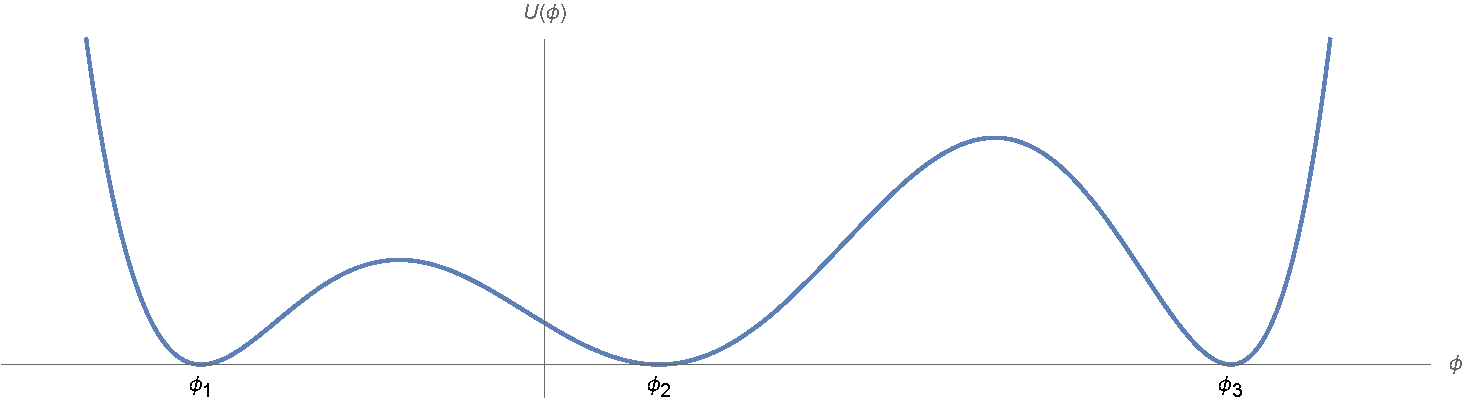
\includegraphics[width=0.75\linewidth]{fig/fig0.pdf}
    \end{figure}

    Consider perturbation theory of $\phi$ around a vacuum, wlog, say $\phi_1$, we can expand it as $\phi = \phi_1 + \delta \phi$ where $\delta \phi$ can be regarded as a ``small'' scalar boson, then 
    \begin{equation}
        \dv{U}{\phi} \simeq \underbrace{\dv{U}{\phi}\bigg|_{\phi_1}}_{0} + \underbrace{\dv[2]{U}{\phi}\bigg|_{\phi_1}}_{m^2} \delta \phi + \underbrace{\cdots}_{\text{neglect}}
    \end{equation}
    where $m$ is identified as the mass of the scalar boson. Here, \eqref{eq:2d-eom} becomes 
    \begin{equation}
        (\square + m^2) \delta \phi = 0,
    \end{equation}
    which is the Klein-Gordon equation.

    In QFT, the perturbation theory leads to Feynman diagrams, infinities, regularisations, ..., and perhaps string theory is called to help with the UV divergences. 

    In contrast, here we consider solitons: the finite energy solutions which end to an element of $U^{-1}(0)$ as $x\to \pm \infty$. These are called \emph{kinks} and they interpolate between the two neighbouring vacuum 
    \begin{equation}
        \begin{split}
            \phi & \to \phi_1 \quad \text{as} \quad x \to -\infty,\\
            \phi & \to \phi_2 \quad \text{as} \quad x \to + \infty.
        \end{split}
    \end{equation}
    \begin{center}
        \tikzset{every picture/.style={line width=0.75pt}} %set default line width to 0.75pt        

        \begin{tikzpicture}[x=0.75pt,y=0.75pt,yscale=-1,xscale=1]
        %uncomment if require: \path (0,300); %set diagram left start at 0, and has height of 300

        %Straight Lines [id:da12203820705850488] 
        \draw    (8.67,97.74) -- (265.03,97.74) ;
        \draw [shift={(267.03,97.74)}, rotate = 180] [color={rgb, 255:red, 0; green, 0; blue, 0 }  ][line width=0.75]    (10.93,-3.29) .. controls (6.95,-1.4) and (3.31,-0.3) .. (0,0) .. controls (3.31,0.3) and (6.95,1.4) .. (10.93,3.29)   ;
        %Straight Lines [id:da4473446345362042] 
        \draw    (121.7,155.69) -- (121.7,32.13) ;
        \draw [shift={(121.7,30.13)}, rotate = 90] [color={rgb, 255:red, 0; green, 0; blue, 0 }  ][line width=0.75]    (10.93,-3.29) .. controls (6.95,-1.4) and (3.31,-0.3) .. (0,0) .. controls (3.31,0.3) and (6.95,1.4) .. (10.93,3.29)   ;
        %Straight Lines [id:da6963367313071676] 
        \draw  [dash pattern={on 0.84pt off 2.51pt}]  (8.67,43.54) -- (267.03,43.54) ;
        %Straight Lines [id:da9521092416166261] 
        \draw  [dash pattern={on 0.84pt off 2.51pt}]  (8.67,149.25) -- (267.03,149.25) ;
        %Curve Lines [id:da6596932304673173] 
        \draw [color={rgb, 255:red, 74; green, 144; blue, 226 }  ,draw opacity=1 ]   (8.67,143.46) .. controls (99.64,143.3) and (113.68,119.37) .. (130.04,95.37) .. controls (146.49,71.24) and (165.28,47.04) .. (267.03,46.87) ;

        % Text Node
        \draw (111.1,22) node    {$\phi $};
        % Text Node
        \draw (280.02,98.41) node    {$x$};
        % Text Node
        \draw (270.46,28.43) node    {$\phi _{+} =\phi _{2}$};
        % Text Node
        \draw (270.26,163.72) node    {$\phi _{-} =\phi _{1}$};


        \end{tikzpicture}
    \end{center}    
    This is a non-perturbative solution as $\phi_1 \neq \phi_2 - \delta \phi$. 

    Static kinks are functions of space only $\phi = \phi(x)$, so \eqref{eq:2d-eom} becomes 
    \begin{equation}
        \phi_{xx} = \dv{U}{\phi}
    \end{equation}
    which is an ODE. Formally, this looks like Newton's equation with ``position'' $\phi$, and ``time'' $x$, in a reversed potential.

    The first integral reads 
    \begin{equation}
        \frac{1}{2} \phi_x^2 - U(\phi) = \text{const.} = 0 
    \end{equation}
    when evaluated at $x = -\infty$, so 
    \begin{equation}
        \int^\phi \frac{\dd{\tilde \phi}}{\sqrt{2 U(\tilde \phi)}} = x - x_0. \label{eq:2d-1st-int}
    \end{equation}

    \begin{ex}
        Consider the following potential 
        \begin{equation}
            U(\phi) = \frac{1}{2} \lambda^2 \left( a^2 - \phi^2 \right)^2
        \end{equation}
        where $\lambda$ is a coupling constant.
        \begin{figure}[H]
            \centering
            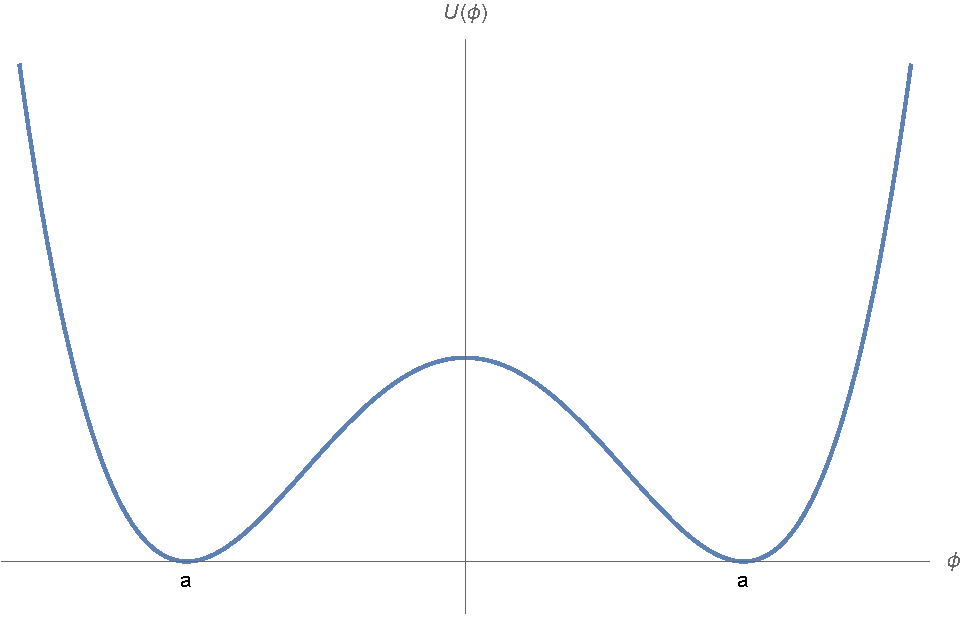
\includegraphics[width=0.5\linewidth]{fig/fig0.1.pdf}
        \end{figure}
        Expand around $\phi = a$, we get 
        \begin{equation}
            U \approx \frac{1}{2} (2 \lambda a)^2 (a - \phi)^2 + \cdots 
        \end{equation}
        so the mass of the scalar boson is $m = 2 \lambda a$. \eqref{eq:2d-1st-int} becomes 
        \begin{equation}
            \underbrace{\pm \frac{1}{\lambda} \int^\phi \frac{\dd{\tilde \phi}}{a^2 - {\tilde \phi}^2}}_{\pm \frac{1}{\lambda a} \tanh^{-1}(\phi / a)} = x - x_0
        \end{equation}
        so 
        \begin{equation}
            \phi_\text{k} = \pm a \tanh(\lambda a (x-x_0))
        \end{equation}
        which interpolates between $\phi = a$ and $\phi = -a$. 

        The mass of the kink is 
        \begin{equation}
            M = E = \int_{-\infty}^{+\infty} \left\{ \frac{1}{2} \phi_x^2 + U(\phi) \right\} \dd{x} = \frac{4}{3} \lambda a^3 \gg m \text{ in perturbation theory}.
        \end{equation}
    \end{ex}

    Moving kinks can be found by Lorentz boosts 
    \begin{equation}
        \phi(t,x) = \phi_\text{k}\left( \gamma(x - v t) \right), \quad \gamma = \frac{1}{\sqrt{1 - v^2}}.
    \end{equation}
    \begin{center}
        \tikzset{every picture/.style={line width=0.75pt}} %set default line width to 0.75pt        
        \begin{tikzpicture}[x=0.75pt,y=0.75pt,yscale=-1,xscale=1]
        %uncomment if require: \path (0,300); %set diagram left start at 0, and has height of 300

        %Straight Lines [id:da1511994200361908] 
        \draw    (8.67,97.74) -- (265.03,97.74) ;
        \draw [shift={(267.03,97.74)}, rotate = 180] [color={rgb, 255:red, 0; green, 0; blue, 0 }  ][line width=0.75]    (10.93,-3.29) .. controls (6.95,-1.4) and (3.31,-0.3) .. (0,0) .. controls (3.31,0.3) and (6.95,1.4) .. (10.93,3.29)   ;
        %Straight Lines [id:da32539115167386745] 
        \draw    (121.7,155.69) -- (121.7,32.13) ;
        \draw [shift={(121.7,30.13)}, rotate = 90] [color={rgb, 255:red, 0; green, 0; blue, 0 }  ][line width=0.75]    (10.93,-3.29) .. controls (6.95,-1.4) and (3.31,-0.3) .. (0,0) .. controls (3.31,0.3) and (6.95,1.4) .. (10.93,3.29)   ;
        %Straight Lines [id:da7605893273359174] 
        \draw  [dash pattern={on 0.84pt off 2.51pt}]  (8.67,43.54) -- (267.03,43.54) ;
        %Straight Lines [id:da3056855051400029] 
        \draw  [dash pattern={on 0.84pt off 2.51pt}]  (8.67,149.25) -- (267.03,149.25) ;
        %Curve Lines [id:da8050010515732298] 
        \draw [color={rgb, 255:red, 74; green, 144; blue, 226 }  ,draw opacity=1 ] [dash pattern={on 4.5pt off 4.5pt}]  (8.67,143.46) .. controls (99.64,143.3) and (113.68,119.37) .. (130.04,95.37) .. controls (146.49,71.24) and (165.28,47.04) .. (267.03,46.87) ;
        %Curve Lines [id:da36009154378883323] 
        \draw [color={rgb, 255:red, 74; green, 144; blue, 226 }  ,draw opacity=1 ]   (8.67,143.46) .. controls (159,140.67) and (151.98,122) .. (168.33,98) .. controls (184.69,74) and (208.33,47.33) .. (267.03,46.87) ;
        %Straight Lines [id:da5952927707308182] 
        \draw [color={rgb, 255:red, 208; green, 2; blue, 27 }  ,draw opacity=1 ]   (140.5,89.92) -- (168,89.99) ;
        \draw [shift={(170,90)}, rotate = 180.16] [color={rgb, 255:red, 208; green, 2; blue, 27 }  ,draw opacity=1 ][line width=0.75]    (10.93,-3.29) .. controls (6.95,-1.4) and (3.31,-0.3) .. (0,0) .. controls (3.31,0.3) and (6.95,1.4) .. (10.93,3.29)   ;

        % Text Node
        \draw (111.1,22) node    {$\phi $};
        % Text Node
        \draw (280.02,98.41) node    {$x$};
        % Text Node
        \draw (270.46,28.43) node    {$\phi _{+} =\phi _{2}$};
        % Text Node
        \draw (270.26,163.72) node    {$\phi _{-} =\phi _{1}$};
        % Text Node
        \draw (156.97,79.95) node  [color={rgb, 255:red, 208; green, 2; blue, 27 }  ,opacity=1 ]  {$t$};


        \end{tikzpicture}
    \end{center}
    





    
    \subsection{Bogomolny Equations}
    \lec{2} We require the field configuration $\phi$ to be elements of $U^{-1}(0)$ as $x\to \pm \infty$, i.e., $\lim_{x \to \pm \infty} \phi = \phi_\pm$
    \begin{center}
        

\tikzset{every picture/.style={line width=0.75pt}} %set default line width to 0.75pt        

\begin{tikzpicture}[x=0.75pt,y=0.75pt,yscale=-1,xscale=1]
%uncomment if require: \path (0,380); %set diagram left start at 0, and has height of 380

%Straight Lines [id:da3971046648421479] 
\draw    (6,93.93) -- (158.79,93.93) ;
\draw [shift={(160.79,93.93)}, rotate = 180] [color={rgb, 255:red, 0; green, 0; blue, 0 }  ][line width=0.75]    (10.93,-3.29) .. controls (6.95,-1.4) and (3.31,-0.3) .. (0,0) .. controls (3.31,0.3) and (6.95,1.4) .. (10.93,3.29)   ;
%Straight Lines [id:da5446186108317181] 
\draw    (73.72,151.88) -- (73.72,28.32) ;
\draw [shift={(73.72,26.32)}, rotate = 90] [color={rgb, 255:red, 0; green, 0; blue, 0 }  ][line width=0.75]    (10.93,-3.29) .. controls (6.95,-1.4) and (3.31,-0.3) .. (0,0) .. controls (3.31,0.3) and (6.95,1.4) .. (10.93,3.29)   ;
%Straight Lines [id:da8899747963646416] 
\draw  [dash pattern={on 0.84pt off 2.51pt}]  (6,43.07) -- (160.79,43.07) ;
%Straight Lines [id:da8836907549162989] 
\draw  [dash pattern={on 0.84pt off 2.51pt}]  (6,145.44) -- (160.79,145.44) ;
%Curve Lines [id:da8976173223361867] 
\draw [color={rgb, 255:red, 74; green, 144; blue, 226 }  ,draw opacity=1 ]   (6,142.23) .. controls (115.32,141.9) and (39.21,45.96) .. (160.79,45.64) ;
%Straight Lines [id:da1118089647958318] 
\draw    (209.16,93.93) -- (361.95,93.93) ;
\draw [shift={(363.95,93.93)}, rotate = 180] [color={rgb, 255:red, 0; green, 0; blue, 0 }  ][line width=0.75]    (10.93,-3.29) .. controls (6.95,-1.4) and (3.31,-0.3) .. (0,0) .. controls (3.31,0.3) and (6.95,1.4) .. (10.93,3.29)   ;
%Straight Lines [id:da8119704281678621] 
\draw    (276.88,151.88) -- (276.88,28.32) ;
\draw [shift={(276.88,26.32)}, rotate = 90] [color={rgb, 255:red, 0; green, 0; blue, 0 }  ][line width=0.75]    (10.93,-3.29) .. controls (6.95,-1.4) and (3.31,-0.3) .. (0,0) .. controls (3.31,0.3) and (6.95,1.4) .. (10.93,3.29)   ;
%Straight Lines [id:da6631481025955495] 
\draw  [dash pattern={on 0.84pt off 2.51pt}]  (209.16,43.07) -- (363.95,43.07) ;
%Straight Lines [id:da1690076949844015] 
\draw  [dash pattern={on 0.84pt off 2.51pt}]  (209.16,145.44) -- (363.95,145.44) ;
%Curve Lines [id:da3358918239778499] 
\draw [color={rgb, 255:red, 74; green, 144; blue, 226 }  ,draw opacity=1 ]   (209.16,45.64) .. controls (342.99,45.96) and (240.44,141.9) .. (363.95,142.23) ;
%Straight Lines [id:da3653858972883368] 
\draw    (412.32,93.93) -- (565.11,93.93) ;
\draw [shift={(567.11,93.93)}, rotate = 180] [color={rgb, 255:red, 0; green, 0; blue, 0 }  ][line width=0.75]    (10.93,-3.29) .. controls (6.95,-1.4) and (3.31,-0.3) .. (0,0) .. controls (3.31,0.3) and (6.95,1.4) .. (10.93,3.29)   ;
%Straight Lines [id:da6500084697998341] 
\draw    (480.04,151.88) -- (480.04,28.32) ;
\draw [shift={(480.04,26.32)}, rotate = 90] [color={rgb, 255:red, 0; green, 0; blue, 0 }  ][line width=0.75]    (10.93,-3.29) .. controls (6.95,-1.4) and (3.31,-0.3) .. (0,0) .. controls (3.31,0.3) and (6.95,1.4) .. (10.93,3.29)   ;
%Straight Lines [id:da8724328450492034] 
\draw  [dash pattern={on 0.84pt off 2.51pt}]  (412.32,43.07) -- (567.11,43.07) ;
%Straight Lines [id:da5611128763195938] 
\draw  [dash pattern={on 0.84pt off 2.51pt}]  (412.32,145.44) -- (567.11,145.44) ;
%Curve Lines [id:da28548957123557117] 
\draw [color={rgb, 255:red, 74; green, 144; blue, 226 }  ,draw opacity=1 ]   (412.32,142.23) .. controls (457.14,142.55) and (433.28,55.62) .. (489.71,55.3) .. controls (546.15,54.98) and (529.91,142.13) .. (567.11,142.23) ;

% Text Node
\draw (61.78,16.86) node    {$\phi $};
% Text Node
\draw (173.36,93.93) node    {$x$};
% Text Node
\draw (158.85,27.29) node    {$\phi _{+} =\phi _{2}$};
% Text Node
\draw (162.72,160.58) node    {$\phi _{-} =\phi _{1}$};
% Text Node
\draw (264.94,16.86) node    {$\phi $};
% Text Node
\draw (376.52,93.93) node    {$x$};
% Text Node
\draw (362.01,27.29) node    {$\phi _{+} =\phi _{2}$};
% Text Node
\draw (365.88,160.58) node    {$\phi _{-} =\phi _{1}$};
% Text Node
\draw (468.1,16.86) node    {$\phi $};
% Text Node
\draw (579.68,93.93) node    {$x$};
% Text Node
\draw (565.17,27.29) node    {$\phi _{+} =\phi _{2}$};
% Text Node
\draw (569.04,160.58) node    {$\phi _{-} =\phi _{1}$};
% Text Node
\draw (78.89,171.68) node   [align=left] {kink};
% Text Node
\draw (286.07,171.2) node   [align=left] {anti-kink};
% Text Node
\draw (186.91,210.8) node    {$\phi _{-} \neq \phi _{+}$};
% Text Node
\draw (188.84,259.58) node   [align=left] {The asymptotic values stay fixed under any\\continuous change of $\displaystyle \phi $. Kinks and antikinks\\are \textit{topologically stable.}};
% Text Node
\draw (486.81,201.14) node    {$\phi _{-} =\phi _{+}$};
% Text Node
\draw (390.75,230.09) node [anchor=north west][inner sep=0.75pt]   [align=left] {Any continuous, finite-energy\\deformation can change the\\field configuration to constant.};
% Connection
\draw    (256.02,183.2) -- (221.32,197.06) ;
\draw [shift={(219.46,197.8)}, rotate = 338.23] [color={rgb, 255:red, 0; green, 0; blue, 0 }  ][line width=0.75]    (10.93,-3.29) .. controls (6.95,-1.4) and (3.31,-0.3) .. (0,0) .. controls (3.31,0.3) and (6.95,1.4) .. (10.93,3.29)   ;
% Connection
\draw    (95.89,177.84) -- (150.03,197.45) ;
\draw [shift={(151.91,198.13)}, rotate = 199.91] [color={rgb, 255:red, 0; green, 0; blue, 0 }  ][line width=0.75]    (10.93,-3.29) .. controls (6.95,-1.4) and (3.31,-0.3) .. (0,0) .. controls (3.31,0.3) and (6.95,1.4) .. (10.93,3.29)   ;

\end{tikzpicture}

    \end{center}
    We can define 
    \begin{equation}
        N = \phi_+ - \phi_- = \int_{\phi_-}^{\phi_+} \dd{\phi} = \int_{-\infty}^{+\infty} \pdv{\phi}{x} \dd{x}
    \end{equation}
    as the \emph{topological charge}. One shows it is conserved. It is \emph{not} associated to any continuous symmetry of $L$ (so, it is not Noether). The field equation (\ref{eq:2d-eom}) did not enter our discussion. Finiteness of energy is the only condition used.
    
    We look for minimal energy configurations for each $N$. As $U \geq 0$, so wlog we write 
    \begin{equation}
        U = \frac{1}{2} \left( \dv{W}{\phi} \right)^2
    \end{equation}
    where $W = W(\phi)$ is called the \emph{superpotential}.

    Now 
    \begin{equation}
        \begin{split}
            E[\phi] & = \frac{1}{2} \int_{-\infty}^{+\infty} \left( \phi_t^2 + \phi_x^2 + W_\phi^2 \right) \dd{x}\\
            & = \frac{1}{2} \int_{-\infty}^{+\infty} \left( \phi_t^2 + \left( \phi_x \mp W_\phi \right)^2 \pm 2 \phi_x W_\phi\right) \dd{x}\\
            & = \frac{1}{2} \int_{-\infty}^{+\infty} \left( \phi_t^2 + \left( \phi_x \mp W_\phi \right)^2 \right) \dd{x} \pm \left( W(\phi_+) - W(\phi_-) \right)\\
        \end{split}
    \end{equation}
    where $W_\phi = \dv{W}{\phi}$. Assuming $\phi_+ \geq \phi_-$ wlog and we take the plus sign in the above equation to get 
    \begin{equation}
        E \geq W(\phi_+) - W(\phi_-).
    \end{equation}
    Without such assumption, we can write more generally 
    \begin{equation}
        E \geq |W(\phi_+) - W(\phi_-)|.
    \end{equation}

    This is known as the \emph{Bogomolny bound}. It depends only on the asymptotic value of $\phi$. The bound is saturated iff 
    \begin{equation}
        \boxed{\pdv{\phi}{t} = 0, \quad \pdv{\phi}{x} = \dv{W}{\phi}}\,. \label{eq:Bogomolny}
    \end{equation}
    These are known as the \emph{Bogomolny equations}. Their solutions are static kinks. Equations (\ref{eq:Bogomolny}) are first-order, but they imply second-order field equations (\ref{eq:2d-eom}).

    The Bogomolny equations for other soliton models are often integrable even if the full Euler-Lagrange equations are not (c.f., Yang-Mills instantons). 

    For example, we go back to $\phi^4$-model, the potential is 
    \begin{equation}
        U = \frac{1}{2} \lambda^2 (a^2 - \phi^2)^2 = \frac{1}{2} \left( \dv{W}{\phi} \right)^2
    \end{equation}
    we choose plus sign and the integration constant as zero, wlog, 
    \begin{equation}
        \dv{W}{\phi} = \lambda (a^2 - \phi^2) \qquad \Rightarrow\qquad W = \lambda \left(a^2 \phi - \frac{\phi^3}{3}\right)
    \end{equation}
    We find the kink energy for $\phi_+ = a, \phi_- = -a$ as 
    \begin{equation}
        E = \lambda \left( a^3 - \frac{a^3}{3} + a^3 - \frac{a^3}{3} \right) = \frac{4}{3} \lambda a^3.
    \end{equation}

    \begin{ex}
        For potential $U(\phi) = 1 - \cos(\beta \phi)$ with $\beta \neq 0$ a constant, the field equation \ref{} gives 
        \begin{equation}
            \phi_{tt} - \phi_{xx} = \beta \sin(\beta \phi)
        \end{equation}
        which is known as the \emph{Sine-Gordon equation}. It has infinitely many vacua with field configuration 
        \begin{equation}
            \phi_n = \frac{2 \pi n}{\beta}.
        \end{equation}
        \begin{figure}[H]
            \centering
            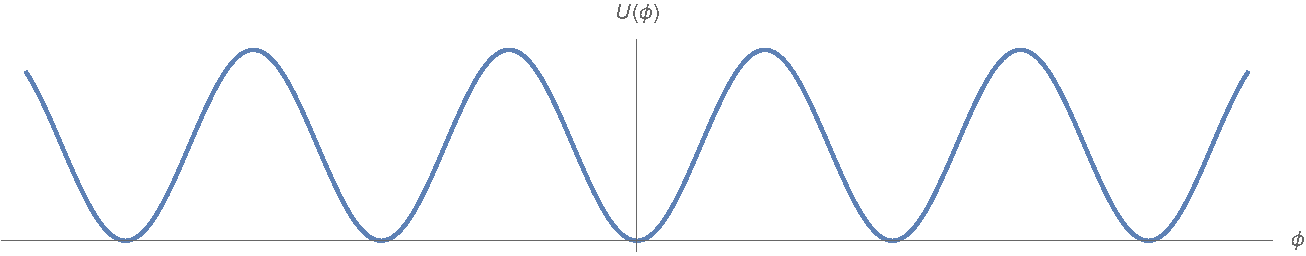
\includegraphics[width=0.75\linewidth]{fig/fig1.pdf}
        \end{figure}
        \label{ex:sine-gordon}
    \end{ex}

    \begin{exer}
        Show that the kinks in example \ref{ex:sine-gordon} is given by 
        \begin{equation}
            \phi(x) = \frac{4}{\beta} \arctan(\exp(\beta (x - x_0))).
        \end{equation}
        Note that this is multivalued, so it encaptures all kinks.
    \end{exer}

    Sine-Gordon is completely integrable (c.f., Part II Integrable Systems), and there exist explicit time-dependent solutions, known as the ``breathers''. It has $\phi_+ - \phi_- = 0$ which is topologically unstable, but dynamically stable.

    \begin{center}
        

\tikzset{every picture/.style={line width=0.75pt}} %set default line width to 0.75pt        

\begin{tikzpicture}[x=0.75pt,y=0.75pt,yscale=-1,xscale=1]
%uncomment if require: \path (0,300); %set diagram left start at 0, and has height of 300

%Straight Lines [id:da42930934687135625] 
\draw    (23.65,98.41) -- (176.44,98.41) ;
\draw [shift={(178.44,98.41)}, rotate = 180] [color={rgb, 255:red, 0; green, 0; blue, 0 }  ][line width=0.75]    (10.93,-3.29) .. controls (6.95,-1.4) and (3.31,-0.3) .. (0,0) .. controls (3.31,0.3) and (6.95,1.4) .. (10.93,3.29)   ;
%Straight Lines [id:da8648520654791672] 
\draw    (91.37,156.36) -- (91.37,32.8) ;
\draw [shift={(91.37,30.8)}, rotate = 90] [color={rgb, 255:red, 0; green, 0; blue, 0 }  ][line width=0.75]    (10.93,-3.29) .. controls (6.95,-1.4) and (3.31,-0.3) .. (0,0) .. controls (3.31,0.3) and (6.95,1.4) .. (10.93,3.29)   ;
%Straight Lines [id:da3627589849572521] 
\draw  [dash pattern={on 0.84pt off 2.51pt}]  (23.65,47.54) -- (178.44,47.54) ;
%Straight Lines [id:da889562533239159] 
\draw  [dash pattern={on 0.84pt off 2.51pt}]  (23.65,149.92) -- (178.44,149.92) ;
%Curve Lines [id:da0034348664464680656] 
\draw [color={rgb, 255:red, 74; green, 144; blue, 226 }  ,draw opacity=1 ]   (23.65,146.7) .. controls (68.48,147.02) and (44.61,60.1) .. (101.05,59.77) .. controls (157.48,59.45) and (141.24,146.6) .. (178.44,146.7) ;

% Text Node
\draw (79.43,21.33) node    {$\phi $};
% Text Node
\draw (191.02,98.41) node    {$x$};
% Text Node
\draw (95.48,173.62) node    {$\phi _{+} -\phi _{-} =0$};
% Text Node
\draw (98.01,198.17) node   [align=left] {``breathers''};


\end{tikzpicture}

    \end{center}

    \subsection{Higher Dimensions and Derrick's Scaling Argument}

    We consider a field $\phi(t, \vb x)$ in $\mathbb{R}^{1,D}$. We are tempted to ask: are there static, finite-energy solutions to the Euler-Lagrange equations below?
    \begin{equation}
        \laplacian \phi = \dv{U}{\phi}.
    \end{equation} 

    These are critical points of the potential energy functional 
    \begin{equation}
        E[\phi] = \int_{\mathbb{R}^D} \left\{ \frac{1}{2} |\grad \phi|^2 + U(\phi) \right\} \dd[D]{\vb x} = E_\text{grad} + E_U.
    \end{equation}

    Assume the $\phi(\vb x)$ is a critical point. Set $\phi_c(\vb x) \equiv \phi(c \vb x)$ so that 
    \begin{equation}
        \tilde{\vb x} = c \vb x, \quad \dd[D]{\tilde{\vb x}} = c^D \dd[D]{\vb x}
    \end{equation}
    and $\phi_1(\vb x) = \phi(\vb x)$ is critical. \lec{3}
    \begin{equation}
        E[\phi_c] = \frac{1}{c^{D-2}} E_\text{grad} + \frac{1}{c^{D}} E_U
    \end{equation}
    \begin{equation}
        \dv{E[\phi_c]}{c}\bigg|_{c=1} = 0 \qquad \Rightarrow\qquad (D-2) E_\text{grad} + D E_U = 0
    \end{equation}
    but note that $E_\text{grad} > 0$ and $E_U \geq 0$. We have the following cases 
    \begin{itemize}
        \item $D=1$, $E_\text{grad} = E_U$ give 1-dim kinks;
        \item $D=2$, $E_U = 0$, in this case, it is possible to get solitons if $\phi: \mathbb{R} \to \Sigma$ has a target manifold with no linear structure, e.g., $\Sigma = S^2$. We will study such solitons: sigma model lumps;
        \item $D=3$, no solitons.
    \end{itemize}

    Ways around Derrick's argument for $D \geq 3$:
    \begin{itemize}
        \item Allow curved backgrounds;
        \item $D=3$: Add the Skyrme term $|\grad \phi|^4$ to the energy integrand, and take $\phi: \mathbb{R}^3 \to S^3 \simeq \SU(2)$ [Skyrmions, describe nuclear physics effectively];
    \end{itemize}

    \subsubsection{Derrick's Argument for Gauge Theories}

    Take a scalar field $\phi : \mathbb{R}^3 \to \mathbb{R}$ and a gauge potential $A = A_\mu(x) \dd{x^\mu}$. We find the field strength (curvature) associated to $A$ as $F \sim \nabla A + A^2$ and the covariant derivative for $\phi$ as $D \phi \sim \nabla \phi + A \phi$.
    
    Now the energy functional of the gauge field is 
    \begin{equation}
        E[A, \phi] = \frac{1}{2} \int_{\mathbb{R}^D} \left\{ F^2 + |D \phi|^2 + U(\phi) \right\} \dd[D]{x} = E_F + E_\text{grad} + E_U
    \end{equation}
    with the three terms all non-negative.

    Assume $(\phi(x), A)$ is a finite $E$ critical point of $E[A, \phi]$ (i.e., soliton). We use the same scaling argument 
    \begin{equation}
        \phi_c = \phi(c x), \quad A_{(c) \mu}(x) = c A_{\mu}(c x), \quad F_{(c) \mu \nu}(x) = c^2 F_{\mu \nu}(c x)
    \end{equation}
    to find that the energy functional scales as 
    \begin{equation}
        E[A_c, \phi_c ] = \frac{1}{c^{D-4}} E_F + \frac{1}{c^{D-2}} E_{\text{grad}} + \frac{1}{c^D} E_U
    \end{equation}
    so at the critical point
    \begin{equation}
        \dv{c} E[A_c, \phi_c] \bigg|_{c=1} = 0 
    \end{equation}
    gives 
    \begin{equation}
        (D-4)E_F + (D-2) E_\text{grad} + D E_U = 0.
    \end{equation}

    \begin{itemize}
        \item $D=1$, there exist gauged kinks;
        \item $D=2$, we need $E_F = E_U$. This is satisfied when we have Abelian vortices in Abelian Higgs model (we will study this later); 
        \item $D=3$, if we switch off the potential term, then we need $E_F = E_\text{grad}$. This occurs when we study non-abelian magnetic monopoles;
        \item $D=4$, we need $E_\text{grad} = E_U = 0$. We have instantons in Yang-Mills theory on $\mathbb{R}^4$ with $E_F \neq 0$ (we will study this as well);
        \item $D > 4$, no solitons. But people study higher forms and branes, where solitons exist...
    \end{itemize}
    \newpage
    \section{Topological Degree of Smooth Maps}
    Look back at the Sine-Gordon model $(\beta = 1)$ 
    \begin{equation}
        \phi_{tt} - \phi_{xx} + \sin \phi = 0
    \end{equation}
    we identify $\phi \sim \phi + 2 n \pi$, so we can think of $\phi$ as $\phi: \mathbb{R} \to S^1$ if static (i.e., no time).

    We consider the following finite energy configuration with asymptotic conditions 
    \begin{equation}
        \phi \to \phi_- = 2 \pi n_- \quad \text{as} \quad x \to -\infty, \qquad \phi \to \phi_+ = 2 \pi n_+ \quad \text{as} \quad x \to +\infty
    \end{equation}
    with $n_-, n_+ \in \mathbb{Z}$ and we define $N = n_+ - n_-$ as the topological charge. 

    If we compactify the space, $\phi$ extends to a map $\phi: S^1 \to S^1$. Such maps are characterised by \emph{winding number}.

    For $f: S^1 \to S^1$, pick $f_0$ which is not a critical value of $f$. Then we define the \emph{degree} of $f$ as 
    \begin{equation}
        \deg (f) = \sum_{\theta: f(\theta) = f_0} \sgn \left( \dv{f}{\theta} \right). \label{eq:deg1}
    \end{equation}
    For example, the function below
    \begin{center}
        

\tikzset{every picture/.style={line width=0.75pt}} %set default line width to 0.75pt        

\begin{tikzpicture}[x=0.75pt,y=0.75pt,yscale=-1,xscale=1]
%uncomment if require: \path (0,300); %set diagram left start at 0, and has height of 300

%Straight Lines [id:da761597142436524] 
\draw    (80,210) -- (268,210) ;
\draw [shift={(270,210)}, rotate = 180] [color={rgb, 255:red, 0; green, 0; blue, 0 }  ][line width=0.75]    (10.93,-3.29) .. controls (6.95,-1.4) and (3.31,-0.3) .. (0,0) .. controls (3.31,0.3) and (6.95,1.4) .. (10.93,3.29)   ;
%Straight Lines [id:da7998280717379076] 
\draw    (90,220) -- (90,36.44) ;
\draw [shift={(90,34.44)}, rotate = 90] [color={rgb, 255:red, 0; green, 0; blue, 0 }  ][line width=0.75]    (10.93,-3.29) .. controls (6.95,-1.4) and (3.31,-0.3) .. (0,0) .. controls (3.31,0.3) and (6.95,1.4) .. (10.93,3.29)   ;
%Straight Lines [id:da727170908878803] 
\draw  [dash pattern={on 0.84pt off 2.51pt}]  (90,60) -- (240,60) ;
%Straight Lines [id:da6456970962063604] 
\draw  [dash pattern={on 0.84pt off 2.51pt}]  (240,60) -- (240,210) ;
%Curve Lines [id:da8559944320085531] 
\draw [color={rgb, 255:red, 74; green, 144; blue, 226 }  ,draw opacity=1 ]   (90,156) .. controls (96.16,151.38) and (97,132.33) .. (109.67,133) .. controls (122.33,133.67) and (121,176.33) .. (136.33,177.67) .. controls (151.67,179) and (153,84) .. (165,60) ;
%Curve Lines [id:da2068386880302091] 
\draw [color={rgb, 255:red, 74; green, 144; blue, 226 }  ,draw opacity=1 ]   (164,210) .. controls (170.16,205.38) and (174.33,137.67) .. (187,136.33) .. controls (199.67,135) and (200.33,171.67) .. (213.67,171.67) .. controls (227,171.67) and (235.67,163) .. (241,153.67) ;
%Straight Lines [id:da4697076190854139] 
\draw [color={rgb, 255:red, 208; green, 2; blue, 27 }  ,draw opacity=1 ] [dash pattern={on 0.84pt off 2.51pt}]  (90.67,147.33) -- (240.67,147.33) ;
%Straight Lines [id:da9811394863832941] 
\draw [color={rgb, 255:red, 208; green, 2; blue, 27 }  ,draw opacity=1 ]   (198.08,147.5) ;
\draw [shift={(198.08,147.5)}, rotate = 0] [color={rgb, 255:red, 208; green, 2; blue, 27 }  ,draw opacity=1 ][fill={rgb, 255:red, 208; green, 2; blue, 27 }  ,fill opacity=1 ][line width=0.75]      (0, 0) circle [x radius= 2.01, y radius= 2.01]   ;
%Straight Lines [id:da30272519707629186] 
\draw [color={rgb, 255:red, 208; green, 2; blue, 27 }  ,draw opacity=1 ]   (179.5,147.67) ;
\draw [shift={(179.5,147.67)}, rotate = 0] [color={rgb, 255:red, 208; green, 2; blue, 27 }  ,draw opacity=1 ][fill={rgb, 255:red, 208; green, 2; blue, 27 }  ,fill opacity=1 ][line width=0.75]      (0, 0) circle [x radius= 2.01, y radius= 2.01]   ;
%Straight Lines [id:da9913538505775463] 
\draw [color={rgb, 255:red, 208; green, 2; blue, 27 }  ,draw opacity=1 ]   (149.08,147.17) ;
\draw [shift={(149.08,147.17)}, rotate = 0] [color={rgb, 255:red, 208; green, 2; blue, 27 }  ,draw opacity=1 ][fill={rgb, 255:red, 208; green, 2; blue, 27 }  ,fill opacity=1 ][line width=0.75]      (0, 0) circle [x radius= 2.01, y radius= 2.01]   ;
%Straight Lines [id:da23858833165806526] 
\draw [color={rgb, 255:red, 208; green, 2; blue, 27 }  ,draw opacity=1 ]   (119.33,147.25) ;
\draw [shift={(119.33,147.25)}, rotate = 0] [color={rgb, 255:red, 208; green, 2; blue, 27 }  ,draw opacity=1 ][fill={rgb, 255:red, 208; green, 2; blue, 27 }  ,fill opacity=1 ][line width=0.75]      (0, 0) circle [x radius= 2.01, y radius= 2.01]   ;
%Straight Lines [id:da22651287438927503] 
\draw [color={rgb, 255:red, 208; green, 2; blue, 27 }  ,draw opacity=1 ]   (95.92,147.08) ;
\draw [shift={(95.92,147.08)}, rotate = 0] [color={rgb, 255:red, 208; green, 2; blue, 27 }  ,draw opacity=1 ][fill={rgb, 255:red, 208; green, 2; blue, 27 }  ,fill opacity=1 ][line width=0.75]      (0, 0) circle [x radius= 2.01, y radius= 2.01]   ;

% Text Node
\draw (89.67,21.33) node    {$f$};
% Text Node
\draw (283,210) node    {$x$};
% Text Node
\draw (74.79,58.87) node    {$2\pi $};
% Text Node
\draw (241.46,221.53) node    {$2\pi $};
% Text Node
\draw (80.79,222.2) node    {$0$};
% Text Node
\draw (100.47,154.51) node  [font=\footnotesize,color={rgb, 255:red, 208; green, 2; blue, 27 }  ,opacity=1 ]  {$+$};
% Text Node
\draw (144.72,138.1) node  [font=\footnotesize,color={rgb, 255:red, 208; green, 2; blue, 27 }  ,opacity=1 ]  {$+$};
% Text Node
\draw (171.97,152.93) node  [font=\footnotesize,color={rgb, 255:red, 208; green, 2; blue, 27 }  ,opacity=1 ]  {$+$};
% Text Node
\draw (128.97,153.6) node  [font=\footnotesize,color={rgb, 255:red, 208; green, 2; blue, 27 }  ,opacity=1 ]  {$-$};
% Text Node
\draw (204.97,139.35) node  [font=\footnotesize,color={rgb, 255:red, 208; green, 2; blue, 27 }  ,opacity=1 ]  {$-$};
% Text Node
\draw (164.86,239.7) node    {$\deg f=1$};


\end{tikzpicture}

    \end{center}
    has degree $\deg(f) = 1 - 1 + 1 + 1 - 1 = 1$.

    Or, we can provide another definition 
    \begin{equation}
        \deg(f) = \frac{1}{\text{Vol}(S^1)} \int_{S^1} \dd{f} = \frac{1}{2 \pi} \int_{0}^{2 \pi} \dv{f}{\theta} \dd{\theta} \label{eq:deg2}
    \end{equation}
    The expression (\ref{eq:deg1}) is an integer, but possibly coordinate dependent; (\ref{eq:deg2}) is coordinate independent, but is it an integer? Let's check it for SG-kink 
    \begin{equation}
        \deg(\phi) = \frac{1}{2 \pi}(\phi(2 \pi) - \phi(0)) = \frac{1}{2 \pi} (2 \pi n_+ - 2 \pi n_-) = n_+ - n_-.
    \end{equation}

    We generalise to manifolds. Assume that $M, M'$ are $D$-dimensional manifolds, which are compact and without boundary (closed, e.g., $S^D$) and oriented. Let $\omega' \in \Lambda^D(M')$ be the volume form on $M'$. Let $f: M \to M'$ be a smooth map. Define \emph{topological degree} for $f$ as
    \begin{equation}
        \int_M f^*(\omega') = \deg(f) \int_{M'} \omega'. \label{eq:deg-f}
    \end{equation} 

    \lec{4}

    Note that $\deg(f)$ is independent on the choice of $\omega$, say 
    \begin{equation}
        \int_{M'} \omega = \int_{M'} \tilde \omega,
    \end{equation}
    then, cohomology theory suggest that $\tilde \omega = \omega + \dd{\alpha}$ where $\alpha \in \Lambda^{D-1}(M')$, then 
    \begin{equation}
        f^*(\tilde{\omega}) = f^*(\omega) + f^*(\dd{\alpha}) = f^*(\omega) + \dd{(f^* \alpha)}
    \end{equation} 
    but 
    \begin{equation}
        \int_M \dd{(f^* \alpha)} = \int_{\partial M} f^* \alpha = 0 \quad \text{for} \quad \partial M = 0
    \end{equation}

    Also, (\ref{eq:deg-f}) is invariant under scalings of $\omega$. But, why is $\deg(f)$ an integer?

    Take open sets $U_k$ with $k=1,2,\cdots$ numbering pre-images such that maps $f: U_k \to f(U_k)$ are one-to-one.

    \begin{center}
        

\tikzset{every picture/.style={line width=0.75pt}} %set default line width to 0.75pt        

\begin{tikzpicture}[x=0.75pt,y=0.75pt,yscale=-1,xscale=1]
%uncomment if require: \path (0,300); %set diagram left start at 0, and has height of 300

%Shape: Polygon Curved [id:ds03397482871940438] 
\draw   (283.66,88.92) .. controls (311.2,76.23) and (390.15,69.46) .. (407.13,81.3) .. controls (424.11,93.15) and (438.34,147.3) .. (407.59,165.07) .. controls (376.83,182.84) and (311.2,203.15) .. (283.66,165.07) .. controls (256.11,127) and (256.11,101.61) .. (283.66,88.92) -- cycle ;
%Shape: Polygon Curved [id:ds857850043362872] 
\draw  [draw opacity=0][fill={rgb, 255:red, 74; green, 144; blue, 226 }  ,fill opacity=0.32 ] (323.59,112.61) .. controls (351.13,99.92) and (356.18,94.84) .. (373.16,106.69) .. controls (390.15,118.53) and (392.9,123.61) .. (362.15,141.38) .. controls (331.39,159.15) and (317.16,154.07) .. (308.9,137.15) .. controls (300.64,120.23) and (296.05,125.3) .. (323.59,112.61) -- cycle ;
%Straight Lines [id:da7228310135718936] 
\draw [color={rgb, 255:red, 139; green, 87; blue, 42 }  ,draw opacity=1 ]   (340,126) ;
\draw [shift={(340,126)}, rotate = 0] [color={rgb, 255:red, 139; green, 87; blue, 42 }  ,draw opacity=1 ][fill={rgb, 255:red, 139; green, 87; blue, 42 }  ,fill opacity=1 ][line width=0.75]      (0, 0) circle [x radius= 2.01, y radius= 2.01]   ;
%Shape: Polygon Curved [id:ds4879361806402265] 
\draw   (77.67,75.33) .. controls (105.21,62.64) and (184.68,67.49) .. (201.67,79.33) .. controls (218.65,91.18) and (205,116.67) .. (209,136.67) .. controls (213,156.67) and (235.67,184) .. (207,197.33) .. controls (178.33,210.67) and (153.7,210.61) .. (128.33,214.67) .. controls (102.97,218.72) and (77.74,195.21) .. (63.66,175.74) .. controls (49.57,156.27) and (50.13,88.03) .. (77.67,75.33) -- cycle ;
%Shape: Polygon Curved [id:ds12004655670914666] 
\draw  [draw opacity=0][fill={rgb, 255:red, 208; green, 2; blue, 27 }  ,fill opacity=0.26 ] (112.33,178) .. controls (120.33,170.67) and (134.66,168.04) .. (148.5,180.02) .. controls (162.33,192) and (141.67,189.33) .. (134.33,202) .. controls (127,214.67) and (113,204.67) .. (107.67,199.33) .. controls (102.33,194) and (104.33,185.33) .. (112.33,178) -- cycle ;
%Shape: Polygon Curved [id:ds3831354080013465] 
\draw  [draw opacity=0][fill={rgb, 255:red, 208; green, 2; blue, 27 }  ,fill opacity=0.26 ] (74.33,135.33) .. controls (82.33,128) and (91.16,120.02) .. (105,132) .. controls (118.84,143.98) and (114.33,153.33) .. (108.33,158) .. controls (102.33,162.67) and (75,162) .. (69.67,156.67) .. controls (64.33,151.33) and (66.33,142.67) .. (74.33,135.33) -- cycle ;
%Shape: Polygon Curved [id:ds9974499814075024] 
\draw  [draw opacity=0][fill={rgb, 255:red, 208; green, 2; blue, 27 }  ,fill opacity=0.26 ] (123.67,94) .. controls (129,88.67) and (130.66,77.38) .. (144.5,89.36) .. controls (158.33,101.33) and (146.33,108) .. (143,115.33) .. controls (139.67,122.67) and (109,114) .. (103.67,108.67) .. controls (98.33,103.33) and (118.33,99.33) .. (123.67,94) -- cycle ;
%Shape: Polygon Curved [id:ds7722140194714393] 
\draw  [draw opacity=0][fill={rgb, 255:red, 208; green, 2; blue, 27 }  ,fill opacity=0.26 ] (164.33,135.33) .. controls (172.33,128) and (174.33,138.67) .. (179,140.67) .. controls (183.67,142.67) and (199.67,148) .. (192.33,160.67) .. controls (185,173.33) and (167,156.67) .. (161.67,151.33) .. controls (156.33,146) and (156.33,142.67) .. (164.33,135.33) -- cycle ;
%Straight Lines [id:da3280981314751501] 
\draw [color={rgb, 255:red, 144; green, 19; blue, 254 }  ,draw opacity=1 ]   (125.67,189) ;
\draw [shift={(125.67,189)}, rotate = 0] [color={rgb, 255:red, 144; green, 19; blue, 254 }  ,draw opacity=1 ][fill={rgb, 255:red, 144; green, 19; blue, 254 }  ,fill opacity=1 ][line width=0.75]      (0, 0) circle [x radius= 2.01, y radius= 2.01]   ;
%Straight Lines [id:da30831528102641137] 
\draw [color={rgb, 255:red, 144; green, 19; blue, 254 }  ,draw opacity=1 ]   (88,145) ;
\draw [shift={(88,145)}, rotate = 0] [color={rgb, 255:red, 144; green, 19; blue, 254 }  ,draw opacity=1 ][fill={rgb, 255:red, 144; green, 19; blue, 254 }  ,fill opacity=1 ][line width=0.75]      (0, 0) circle [x radius= 2.01, y radius= 2.01]   ;
%Straight Lines [id:da464686413777198] 
\draw [color={rgb, 255:red, 144; green, 19; blue, 254 }  ,draw opacity=1 ]   (174.33,149.33) ;
\draw [shift={(174.33,149.33)}, rotate = 0] [color={rgb, 255:red, 144; green, 19; blue, 254 }  ,draw opacity=1 ][fill={rgb, 255:red, 144; green, 19; blue, 254 }  ,fill opacity=1 ][line width=0.75]      (0, 0) circle [x radius= 2.01, y radius= 2.01]   ;
%Straight Lines [id:da12877025335398384] 
\draw [color={rgb, 255:red, 144; green, 19; blue, 254 }  ,draw opacity=1 ]   (131,103) ;
\draw [shift={(131,103)}, rotate = 0] [color={rgb, 255:red, 144; green, 19; blue, 254 }  ,draw opacity=1 ][fill={rgb, 255:red, 144; green, 19; blue, 254 }  ,fill opacity=1 ][line width=0.75]      (0, 0) circle [x radius= 2.01, y radius= 2.01]   ;
%Curve Lines [id:da6000743803568003] 
\draw [color={rgb, 255:red, 65; green, 117; blue, 5 }  ,draw opacity=1 ]   (138.67,101.5) .. controls (192.13,89.62) and (291.32,102.24) .. (333.09,124.49) ;
\draw [shift={(334.33,125.17)}, rotate = 208.94] [color={rgb, 255:red, 65; green, 117; blue, 5 }  ,draw opacity=1 ][line width=0.75]    (10.93,-3.29) .. controls (6.95,-1.4) and (3.31,-0.3) .. (0,0) .. controls (3.31,0.3) and (6.95,1.4) .. (10.93,3.29)   ;
%Curve Lines [id:da7268807591508393] 
\draw [color={rgb, 255:red, 65; green, 117; blue, 5 }  ,draw opacity=1 ]   (181,148.5) .. controls (235.18,155.07) and (296.79,145.79) .. (333.98,131.17) ;
\draw [shift={(335.67,130.5)}, rotate = 157.93] [color={rgb, 255:red, 65; green, 117; blue, 5 }  ,draw opacity=1 ][line width=0.75]    (10.93,-3.29) .. controls (6.95,-1.4) and (3.31,-0.3) .. (0,0) .. controls (3.31,0.3) and (6.95,1.4) .. (10.93,3.29)   ;
%Curve Lines [id:da7457339185815965] 
\draw [color={rgb, 255:red, 65; green, 117; blue, 5 }  ,draw opacity=1 ]   (95.67,140.83) .. controls (154.7,106.01) and (255.32,108.47) .. (332.83,127.87) ;
\draw [shift={(334,128.17)}, rotate = 194.21] [color={rgb, 255:red, 65; green, 117; blue, 5 }  ,draw opacity=1 ][line width=0.75]    (10.93,-3.29) .. controls (6.95,-1.4) and (3.31,-0.3) .. (0,0) .. controls (3.31,0.3) and (6.95,1.4) .. (10.93,3.29)   ;
%Curve Lines [id:da3781595909535047] 
\draw [color={rgb, 255:red, 65; green, 117; blue, 5 }  ,draw opacity=1 ]   (133,187.17) .. controls (191.74,178.59) and (304.06,173.27) .. (338.64,133.39) ;
\draw [shift={(339.67,132.17)}, rotate = 129.11] [color={rgb, 255:red, 65; green, 117; blue, 5 }  ,draw opacity=1 ][line width=0.75]    (10.93,-3.29) .. controls (6.95,-1.4) and (3.31,-0.3) .. (0,0) .. controls (3.31,0.3) and (6.95,1.4) .. (10.93,3.29)   ;

% Text Node
\draw (375.8,149.2) node  [color={rgb, 255:red, 74; green, 144; blue, 226 }  ,opacity=1 ]  {$V$};
% Text Node
\draw (344.79,61.53) node    {$M'$};
% Text Node
\draw (353.56,122.53) node  [color={rgb, 255:red, 139; green, 87; blue, 42 }  ,opacity=1 ]  {$\mathbf{y}$};
% Text Node
\draw (75.67,117.19) node  [color={rgb, 255:red, 208; green, 2; blue, 27 }  ,opacity=1 ]  {$U_{4}$};
% Text Node
\draw (156.34,200.19) node  [color={rgb, 255:red, 208; green, 2; blue, 27 }  ,opacity=1 ]  {$U_{1}$};
% Text Node
\draw (157.01,82.85) node  [color={rgb, 255:red, 208; green, 2; blue, 27 }  ,opacity=1 ]  {$U_{3}$};
% Text Node
\draw (188.01,131.19) node  [color={rgb, 255:red, 208; green, 2; blue, 27 }  ,opacity=1 ]  {$U_{2}$};
% Text Node
\draw (131.1,53.2) node    {$M$};
% Text Node
\draw (117.98,195.02) node  [color={rgb, 255:red, 144; green, 19; blue, 254 }  ,opacity=1 ]  {$p_{1}$};
% Text Node
\draw (166.31,157.35) node  [color={rgb, 255:red, 144; green, 19; blue, 254 }  ,opacity=1 ]  {$p_{2}$};
% Text Node
\draw (141.64,113.02) node  [color={rgb, 255:red, 144; green, 19; blue, 254 }  ,opacity=1 ]  {$p_{3}$};
% Text Node
\draw (101.64,151.02) node  [color={rgb, 255:red, 144; green, 19; blue, 254 }  ,opacity=1 ]  {$p_{4}$};
% Text Node
\draw (241.89,85.03) node  [color={rgb, 255:red, 65; green, 117; blue, 5 }  ,opacity=1 ]  {$f$};


\end{tikzpicture}

    \end{center}

    Assume that $y$ is generic (not a critical point of $f$). Take $x^1, \cdots, x^D$ as the coordinates on $U_1$, $y^1, \cdots, y^D$ as the coordinates on $f(U_1) \subset V$. 

    Then we can construct the Jacobian matrix
    \begin{equation}
        J = \pdv{y^i}{x^j}
    \end{equation}
    which is a $D\times D$ non-singular matrix.

    Take $\omega$ to be compactly supported on $\bigcap_k f(U_k) \subset V$ i.e., $\omega \equiv 0$ outside this set. Then, 
    \begin{thm}
        $\deg(f)$ is an integer given by 
        \begin{equation}
            \deg(f) = \sum_{p_k: f(p_k) = y} \sgn\left( \det J \right)\label{eq:deg-int}
        \end{equation}
    \end{thm}
    \begin{proof}[Sketch of proof]
        Take 
        \begin{equation}
            \omega = \rho(y) \dd{y^1} \wedge \dd{y^2} \wedge \cdots \wedge \dd{y^D}
        \end{equation}
        and by $f^*(\dd{y^k}) = \pdv{y^k}{x^j} \dd{x^j}$ we have 
        \begin{equation}
            \int_{U_1} f^*(\omega) = \int_{U_1} \rho(f(x)) \det J \dd{x^1} \wedge \dd{x^2} \wedge \cdots \wedge \dd{x^D}.
        \end{equation} 

        Now we change coordinates to $x=x(y)$ 
        \begin{equation}
            \int_{U_1} f^*(\omega) = \sgn{\det J} \int_{M'} \tilde \omega
        \end{equation}
        as the change of coordinates introduce $1/|J|$. 
        
        Repeat this for all points $p_2, \cdots, p_N$ to establish (\ref{eq:deg-int}).
    \end{proof}

    \begin{ex}
        $f: S^2 \to S^2 \subset \mathbb{R}^3$ so $f \in \mathbb{R}^3$, $|f|=1$ and we can denote $f=(f^1,f^2,f^3)$. Then, 
        \begin{equation}
            \deg(f) = \frac{1}{\text{Vol}(S^2)} \times \frac{1}{2} \int \epsilon^{abc} f^a \dd{f^b} \wedge \dd{f^c}. \label{eq:S2-S2}
        \end{equation}

        If $(x^1,x^2)$ are coordinates of $S^2$ (e.g., $(x^1,x^2) = (\phi,\theta)$) then 
        \begin{equation}
            \deg(f) = \frac{1}{8 \pi} \int_{S^2} \epsilon^{abc} f^a \pdv{f^b}{x^i} \pdv{f^c}{x^j} \epsilon^{ij} \dd[2]{x}
        \end{equation}
        where 
        \begin{equation}
            \epsilon^{ij} = \mqty(0 & 1\\-1 & 0).
        \end{equation}
    \end{ex}
    \begin{ex}
        $f: M \to S^3 \simeq \SU(2)$ where $M$ is a closed 3-manifold. $A \in \SU(2)$ if $A^{\dagger} A = \1$, $\det A = 1$. Then 
        \begin{equation}
            \deg(f) = \frac{1}{24 \pi} \int_M \Tr\left( [f^{-1} \dd{f}]^3 \right) \label{eq:su-2}
        \end{equation}
    \end{ex}
    \newpage 
    \section{Sigma Model and Lumps}
    Consider a field 
    \begin{equation}
        \phi : \mathbb{R}^{2,1} \to S^{N-1} \subset \mathbb{R}^N, \quad \phi = (\phi^1,\cdots,\phi^N), \quad |\phi|^2 = \sum_a \phi^a \phi^a = 1.
    \end{equation}
    The Lagrangian density of the theory is 
    \begin{equation}
        \mathcal{L} = \sum_a \frac{1}{2} \eta^{\mu \nu} \pdv{\phi^a}{x^\mu} \pdv{\phi^a}{x^\nu}.
    \end{equation}

    To treat the constraints, we can either 
    
    1) Introduce a Lagrange multiplier to impose the constraint
    \begin{equation}
        \mathcal{L}' = \mathcal{L} - \frac{1}{2} \lambda (1 - |\phi|^2) 
    \end{equation}
    and the Euler-Lagrange equation for $\mathcal{L}'$ is 
    \begin{equation}
        \square \phi^a - \lambda \phi^a = 0.
    \end{equation}
    Contracting with $\phi^a$ we can find the value for $\lambda$ as 
    \begin{equation}
        \lambda = \sum_a \phi^a \square \phi^a
    \end{equation}
    to get 
    \begin{equation}
        \square \phi^a - \left( \sum_b \phi^b \square \phi^b \right) \phi^a = 0 \label{eq:sigma-eom}
    \end{equation}
    which is a system of non-linear PDEs.

    or 2) Substitute the constraint via 
    \begin{equation}
        \phi^N = \pm \sqrt{1 - \sum_p^{N-1} \phi^p \phi^p}
    \end{equation}
    to get 
    \begin{equation}
        \mathcal{L} = \sum_{p,q}\frac{1}{2} g_{pq}(\phi) \eta^{\mu \nu} \pdv{\phi^p}{x^\mu} \pdv{\phi^q}{x^\nu} \label{eq:NLSM}
    \end{equation}
    where 
    \begin{equation}
        g_{pq} = \delta_{pq} + \frac{\phi_p \phi_q}{1 - \sum_{r=1}^{N-1} \phi^r \phi^r}
    \end{equation}
    is a round metric on $S^{N-1}$.

    \begin{rmk}
        (\ref{eq:NLSM}) is a framework for field theories $\phi: (\Sigma, \eta) \to (M,g)$. For example, 
        \begin{enumerate}
            \item If $\Sigma$ is a Riemann surface, $(M,g)$ is a 10-dimensional Lorentzian manifold, then (\ref{eq:NLSM}) is the worldsheet Lagrangian of String Theory.
            \item If $\Sigma = \mathbb{R}$, then (\ref{eq:NLSM}) is the geodesic Lagrangian on $(M,g)$. The integral curves of Euler-Lagrange equations are geodesics. 
            \item How about $\dim(\Sigma) = k > 2$? These are $(k-1)$-branes.
        \end{enumerate}
    \end{rmk}

    \lec{5}
    Now look at the case $N=3$. We are looking for static, finite energy solutions to equation (\ref{eq:sigma-eom})
    \begin{equation}
        \Delta \phi^a - \left( \sum_b \phi^b \Delta \phi^b \right) \phi^a = 0
    \end{equation}
    where $\Delta = \partial_1^2 + \partial_2^2$ and $\phi: \mathbb{R}^2 \to S^2$.

    The energy functional is 
    \begin{equation}
        E[\phi] = \frac{1}{2} \int_{\mathbb{R}^2} |\grad \phi|^2 \dd[2]{\vb x} = \frac{1}{2} \int_{\mathbb{R}^2} \partial_i \phi^a \partial_i \phi^a \dd[2]{x}.
    \end{equation}

    Now we we use the coordinate transformation $x^1 + \mathrm{i} x^2 = r e^{\mathrm{i} \theta}$ and impose a boundary condition $r|\grad \phi| \to 0$ as $r \to \infty$ to avoid the logarithmic blow-up at infinity, so 
    \begin{equation}
        \lim_{r \to \infty} \phi = \phi_\infty = \text{const.} = (0,0,1)
    \end{equation}
    wlog by rotating the target $S^2$. So $\phi$ extends to a one-point compactification $S^2 = \mathbb{R}^2 + \left\{ \infty \right\}$ with $\phi(\infty) \equiv \phi_\infty$. So now we can think of it as $\phi : S^2 \to S^2$. Such maps are partially characterised by their topological degree as in (\ref{eq:S2-S2})
    \begin{equation}
        \deg(\phi) = \frac{1}{8 \pi} \int_{S^2} \epsilon^{ij} \epsilon^{abc} \phi^a \pdv{\phi^b}{x^i} \pdv{\phi^c}{x^j} \dd[2]{x}.
    \end{equation}

    \begin{thm}
        The energy of soliton solutions to (\ref{eq:sigma-eom}) is bounded from below 
        \begin{equation}
            E[\phi] \geq 4 \pi \abs{\deg{\phi}}
        \end{equation}
        with equality if $\phi$ satisfies 1st order Bogomolny equations
        \begin{equation}
            \partial_i \phi^a = \pm \epsilon^{abc} \epsilon_{ij} \phi^b \pdv{\phi^c}{x^j}. \label{eq:NLSM-Bogo}
        \end{equation}
    \end{thm}

    \begin{proof}
        Consider the inequality 
        \begin{equation}
            \begin{split}
                0 \leq \int_{S^2} \left( \partial_i \phi^a \mp \epsilon^{abc} \epsilon_{ij} \phi^b \pdv{\phi^c}{x^j} \right) \left( \partial_i \phi^a \mp \epsilon^{apq} \epsilon_{ik} \phi^p \pdv{\phi^q}{x^k} \right) \dd[2]{x}
            \end{split}
        \end{equation}
        To expand the total square, we use $\phi^a \phi^a = 1$ so $\phi^a \partial_i \phi^a = 0$ and the identities $\epsilon_{ij} \epsilon_{ik} = \delta_{jk}$ for $\epsilon_{ij} = \smqty(0 & 1\\-1 & 0)$ and $\epsilon^{abc} \epsilon^{apq} = \delta^{bp} \delta^{cq} - \delta^{bq} \delta^{cp}$. Then we have, by picking the minus sign,
        \begin{equation}
            \begin{split}
                0 &\leq \int_{S^2} \Bigg( \partial_i \phi^a \partial_i \phi^a - 2 \epsilon^{apq} \epsilon_{ik} \phi^p \pdv{\phi^a}{x_i} \pdv{\phi^q}{x^k} + \underbrace{(\delta^{bp} \delta^{cq} - \delta^{bq} \delta^{cp}) \delta_{jk} \phi^b \phi^p \pdv{\phi^c}{x^j} \pdv{\phi^q}{x^k}}_{\partial_i \phi^c \partial_i \phi^c - 0}  \Bigg) \dd[2]{x}\\
                0 & \leq 4 E - 16 \pi \deg(\phi)
            \end{split}
        \end{equation}
        with equality if (\ref{eq:NLSM-Bogo}) holds with plus sign.
    \end{proof}

    \begin{rmk} ~
        \begin{enumerate}[1)]
            \item Any solution to 1st order equation (\ref{eq:NLSM-Bogo}) is an absolute energy minimizer within a given topological class, so is a solution to (\ref{eq:sigma-eom});
            \item Uhlenbeck (1984): there are no solutions of (\ref{eq:sigma-eom}) with finite energy which do not arise from (\ref{eq:NLSM-Bogo});
            \item (\ref{eq:NLSM-Bogo}) are completely solvable using complex numbers (c.f., exercise) by identifying $S^2 \simeq \mathbb{CP}^1$ (1D complex manifold) via stereographic projection. 
            \begin{center}
                \tikzset{every picture/.style={line width=0.75pt}} %set default line width to 0.75pt        

                \begin{tikzpicture}[x=0.75pt,y=0.75pt,yscale=-1,xscale=1]
                %uncomment if require: \path (0,300); %set diagram left start at 0, and has height of 300

                %Shape: Arc [id:dp8828432850542227] 
                \draw  [draw opacity=0] (250,125) .. controls (250,125) and (250,125) .. (250,125) .. controls (250,125) and (250,125) .. (250,125) .. controls (250,108.43) and (282.83,95) .. (323.33,95) .. controls (363.83,95) and (396.67,108.43) .. (396.67,125) -- (323.33,125) -- cycle ; \draw   (250,125) .. controls (250,125) and (250,125) .. (250,125) .. controls (250,125) and (250,125) .. (250,125) .. controls (250,108.43) and (282.83,95) .. (323.33,95) .. controls (363.83,95) and (396.67,108.43) .. (396.67,125) ;  
                %Straight Lines [id:da12886094679208027] 
                \draw [color={rgb, 255:red, 74; green, 144; blue, 226 }  ,draw opacity=1 ]   (330,40) -- (290,80) ;
                %Straight Lines [id:da14473264000487762] 
                \draw [color={rgb, 255:red, 74; green, 144; blue, 226 }  ,draw opacity=1 ]   (220,150) -- (170,200) ;
                %Shape: Arc [id:dp454618766161343] 
                \draw  [draw opacity=0] (396.67,125) .. controls (396.67,125) and (396.67,125) .. (396.67,125) .. controls (396.67,166.42) and (363.83,200) .. (323.33,200) .. controls (282.83,200) and (250,166.42) .. (250,125) -- (323.33,125) -- cycle ; \draw   (396.67,125) .. controls (396.67,125) and (396.67,125) .. (396.67,125) .. controls (396.67,166.42) and (363.83,200) .. (323.33,200) .. controls (282.83,200) and (250,166.42) .. (250,125) ;  
                %Shape: Parallelogram [id:dp9081876199929055] 
                \draw  [fill={rgb, 255:red, 255; green, 255; blue, 255 }  ,fill opacity=0.75 ] (199,90) -- (530,90) -- (451,170) -- (120,170) -- cycle ;
                %Shape: Arc [id:dp6826281033806154] 
                \draw  [draw opacity=0][fill={rgb, 255:red, 255; green, 255; blue, 255 }  ,fill opacity=0.75 ] (250,125) .. controls (250,83.58) and (282.83,50) .. (323.33,50) .. controls (363.83,50) and (396.67,83.58) .. (396.67,125) -- (323.33,125) -- cycle ; \draw   (250,125) .. controls (250,83.58) and (282.83,50) .. (323.33,50) .. controls (363.83,50) and (396.67,83.58) .. (396.67,125) ;  
                %Shape: Arc [id:dp6065389829585446] 
                \draw  [draw opacity=0] (396.67,125) .. controls (396.67,125) and (396.67,125) .. (396.67,125) .. controls (396.67,125) and (396.67,125) .. (396.67,125) .. controls (396.67,141.57) and (363.83,155) .. (323.33,155) .. controls (282.83,155) and (250,141.57) .. (250,125) -- (323.33,125) -- cycle ; \draw   (396.67,125) .. controls (396.67,125) and (396.67,125) .. (396.67,125) .. controls (396.67,125) and (396.67,125) .. (396.67,125) .. controls (396.67,141.57) and (363.83,155) .. (323.33,155) .. controls (282.83,155) and (250,141.57) .. (250,125) ;  
                %Straight Lines [id:da7438745520788073] 
                \draw [color={rgb, 255:red, 208; green, 2; blue, 27 }  ,draw opacity=1 ]   (320,50) ;
                \draw [shift={(320,50)}, rotate = 0] [color={rgb, 255:red, 208; green, 2; blue, 27 }  ,draw opacity=1 ][fill={rgb, 255:red, 208; green, 2; blue, 27 }  ,fill opacity=1 ][line width=0.75]      (0, 0) circle [x radius= 3.35, y radius= 3.35]   ;
                %Straight Lines [id:da8704780505586467] 
                \draw [color={rgb, 255:red, 74; green, 144; blue, 226 }  ,draw opacity=1 ]   (290,80) -- (220,150) ;
                \draw [shift={(220,150)}, rotate = 135] [color={rgb, 255:red, 74; green, 144; blue, 226 }  ,draw opacity=1 ][fill={rgb, 255:red, 74; green, 144; blue, 226 }  ,fill opacity=1 ][line width=0.75]      (0, 0) circle [x radius= 3.35, y radius= 3.35]   ;
                \draw [shift={(290,80)}, rotate = 135] [color={rgb, 255:red, 74; green, 144; blue, 226 }  ,draw opacity=1 ][fill={rgb, 255:red, 74; green, 144; blue, 226 }  ,fill opacity=1 ][line width=0.75]      (0, 0) circle [x radius= 3.35, y radius= 3.35]   ;

                % Text Node
                \draw (330,100.4) node [anchor=north west][inner sep=0.75pt]    {$S_{d}$};
                % Text Node
                \draw (431,141.4) node [anchor=north west][inner sep=0.75pt]    {$\mathbb{R}^{d}$};
                % Text Node
                \draw (331,30) node [anchor=north west][inner sep=0.75pt]  [color={rgb, 255:red, 208; green, 2; blue, 27 }  ,opacity=1 ] [align=left] {point at $\displaystyle \infty $};
                % Text Node
                \draw (127,206.33) node [anchor=north west][inner sep=0.75pt]  [color={rgb, 255:red, 74; green, 144; blue, 226 }  ,opacity=1 ] [align=left] {stereographic map};


                \end{tikzpicture}
            \end{center}
            In patch $U \subset S^2$, where $\phi \neq (0,0,1)$ \begin{equation}
                f = \frac{\phi^1 - \mathrm{i} \phi^2}{1 - \phi^3} \in \mathbb{C}
            \end{equation}
            and in $\tilde U \subset S^2$ where $\phi \neq (0,0,-1)$ 
            \begin{equation}
                \tilde f = \frac{\phi^1 + \mathrm{i} \phi^2}{1 + \phi^3}.
            \end{equation}
            On $U \cap \tilde U$, $f \tilde f = 1$ so $\tilde f = 1/f$ on $U \cap \tilde U$ holomorphic. 
            \begin{exer}
                Prove that equation (\ref{eq:sigma-eom}) $\Leftrightarrow \bar \partial f = 0$ where $z = x^1 + \mathrm{i} x^2$ where $\bar \partial = \frac{1}{2}(\partial_1 + \mathrm{i} \partial_2)$.  
            \end{exer} 
            Finite energy solutions are rational maps $f: \mathbb{CP}^1 \to \mathbb{CP}^1$, $f = P(z)/Q(z)$ where $P,Q$ are polynomials.
        \end{enumerate}
       
    \end{rmk}
    \newpage
    \section{Abelian Higgs Model}
    
    \lec{6} Consider Abelian Higgs model in 2 spatial dimensions. It contains 
    \begin{itemize}
        \item A complex-valued scalar field \begin{equation}
            \phi : \mathbb{R}^{2,1} \to \mathbb{C} \quad \text{(Higgs field)}
        \end{equation}
        \item An real-valued abelian $\U(1)$ gauge potential \begin{equation}
            A_\mu = (A_0, A_1, A_2) 
        \end{equation}
        and its field strength 
        \begin{equation}
            F_{\mu \nu} = \partial_\mu A_\nu - \partial_\nu A_\mu.
        \end{equation}
    \end{itemize}
    Under a gauge transformation 
    \begin{equation}
        \phi \mapsto e^{\mathrm{i} \alpha} \phi, \quad A_\mu \mapsto A_\mu + \partial_\mu \alpha, \quad F_{\mu \nu} \mapsto F_{\mu \nu}, \quad \alpha : \mathbb{R}^{2,1} \to \mathbb{R}.
    \end{equation}
    We define the covariant derivative 
    \begin{equation}
        D_\mu = \partial_\mu \phi - \mathrm{i} A_\mu \phi
    \end{equation}
    so that 
    \begin{equation}
        D_\mu (e^{\mathrm{i} \alpha}\phi) = e^{\mathrm{i} \alpha} D_\mu \phi.
    \end{equation}

    The Lagrangian for this model reads 
    \begin{equation}
        L = \int_{\mathbb{R}^2} \left\{ - \frac{1}{4} F_{\mu \nu} F^{\mu \nu} + \overline{D_\mu \phi} D^\mu \phi - \frac{\lambda}{8} \left( 1 - \abs{\phi}^2 \right)^2 \right\} \dd[2]{x}
    \end{equation}
    where $\lambda$ is a coupling constant with categorisation 
    \begin{equation}
        \lambda \begin{cases}
            > 1 & \text{Type II superconductor},\\
            < 1 & \text{Type I superconductor},\\
            =1 & \text{critical coupling}.
        \end{cases}
    \end{equation}

    The Euler-Lagrange equations are 
    \begin{equation}
        \begin{dcases}
            D_\mu F^{\mu \nu} = \frac{\mathrm{i}}{2} \left( \overline{D^\nu \phi} \cdot \phi - D^\nu \phi \cdot \phi \right),\\
            D_\mu D^\mu \phi = \frac{\lambda}{2} \left( 1 - \abs{\phi}^2 \right) \phi.
        \end{dcases}
        \label{eq:AHM-eom}
    \end{equation}

    We now want to find static, finite-energy solutions to \eqref{eq:AHM-eom}. First, we introduce the following notations 
    \begin{equation}
        A = A_1 \dd{x^1} + A_2 \dd{x^2}, \quad F = \dd{A} = (\partial_1 A_2 - \partial_2 A_1) \dd{x^1} \wedge \dd{x^2} = F_{12} \dd{x^1} \wedge \dd{x^2} = B \dd{x^1} \wedge \dd{x^2}
    \end{equation}
    where $B$ is the abelian magnetic field. 

    The energy functional is 
    \begin{equation}
        E[\phi,A] = \frac{1}{2} \int_{\mathbb{R}^2}\left\{ B^2 + \overline{D_1 \phi} D_1 \phi + \overline{D_2 \phi} D_2 \phi + \frac{\lambda}{4}\left( 1 - \abs{\phi}^2 \right)^2 \right\} \dd[2]{x}. \label{eq:vtx-E}
    \end{equation}

    Introduce plane polars 
    \begin{equation}
        x^1 = r \cos \theta, \quad x^2 = r \sin \theta
    \end{equation} 
    we find 
    \begin{equation}
        A = A_1(-\sin \theta r \dd{\theta} + \cos \theta \dd{r}) + A_2 (r \cos \theta \dd{\theta} + \sin \theta \dd{r}) = A_r \dd{r} + A_\theta \dd{\theta}
    \end{equation}
    where 
    \begin{equation}
        A_r = \frac{1}{r} \left( A_1 x^1 + A_2 x^2 \right), \quad A_\theta = A_2 x^1 - A_1 x^2.
    \end{equation}
    Then the field strength becomes 
    \begin{equation}
        F = B \dd{x^1} \wedge \dd{x^2} = B r \dd{r} \wedge \dd{\theta} = F_{r \theta} \dd{r} \wedge \dd{\theta}
    \end{equation}
    giving 
    \begin{equation}
        B = \frac{F_{r \theta}}{r}.
    \end{equation}

    In such coordinates, the energy functional \eqref{eq:vtx-E} becomes 
    \begin{equation}
        E[\phi,A] = \frac{1}{2} \int_{\mathbb{R}^2} \left\{ \frac{F_{r \theta}^2}{r^2} + \overline{D_r \phi} D_r \phi + \frac{1}{r^2} \overline{D_\theta \phi} D_\theta \phi + \frac{\lambda}{4} \left( 1 - \abs{\phi}^2 \right)^2 \right\} r \dd{r} \dd{\theta}
    \end{equation}
    and we want it to be finite. Hence, we impose boundary conditions at infinity
    \begin{equation}
        B \to 0, \quad D \phi \to 0, \quad \abs{\phi} \to 1.
    \end{equation} 

    Such finite energy solutions to \eqref{eq:vtx-E} are called \emph{vortices}, they are located at regions where $(\phi, A)$ depart from their asymptotic values. 

    \begin{center}
        

% Gradient Info
  
\tikzset {_34l57e8nl/.code = {\pgfsetadditionalshadetransform{ \pgftransformshift{\pgfpoint{0 bp } { 0 bp }  }  \pgftransformscale{1 }  }}}
\pgfdeclareradialshading{_iz6ksu5xt}{\pgfpoint{0bp}{0bp}}{rgb(0bp)=(0.82,0.01,0.11);
rgb(0bp)=(0.82,0.01,0.11);
rgb(25bp)=(1,1,1);
rgb(400bp)=(1,1,1)}
\tikzset{_mkh1qbti7/.code = {\pgfsetadditionalshadetransform{\pgftransformshift{\pgfpoint{0 bp } { 0 bp }  }  \pgftransformscale{1 } }}}
\pgfdeclareradialshading{_06x3feji6} { \pgfpoint{0bp} {0bp}} {color(0bp)=(transparent!25);
color(0bp)=(transparent!25);
color(25bp)=(transparent!0);
color(400bp)=(transparent!0)} 
\pgfdeclarefading{_7h9545ta2}{\tikz \fill[shading=_06x3feji6,_mkh1qbti7] (0,0) rectangle (50bp,50bp); } 

% Gradient Info
  
\tikzset {_l5gsnr4al/.code = {\pgfsetadditionalshadetransform{ \pgftransformshift{\pgfpoint{0 bp } { 0 bp }  }  \pgftransformscale{1 }  }}}
\pgfdeclareradialshading{_jqnpja0sj}{\pgfpoint{0bp}{0bp}}{rgb(0bp)=(0.82,0.01,0.11);
rgb(0bp)=(0.82,0.01,0.11);
rgb(25bp)=(1,1,1);
rgb(400bp)=(1,1,1)}
\tikzset{_ge9e9fmjl/.code = {\pgfsetadditionalshadetransform{\pgftransformshift{\pgfpoint{0 bp } { 0 bp }  }  \pgftransformscale{1 } }}}
\pgfdeclareradialshading{_hg3as1sjp} { \pgfpoint{0bp} {0bp}} {color(0bp)=(transparent!25);
color(0bp)=(transparent!25);
color(25bp)=(transparent!0);
color(400bp)=(transparent!0)} 
\pgfdeclarefading{_9qq4lv6wi}{\tikz \fill[shading=_hg3as1sjp,_ge9e9fmjl] (0,0) rectangle (50bp,50bp); } 

% Gradient Info
  
\tikzset {_a77w2i35s/.code = {\pgfsetadditionalshadetransform{ \pgftransformshift{\pgfpoint{0 bp } { 0 bp }  }  \pgftransformscale{1 }  }}}
\pgfdeclareradialshading{_b0d19gx41}{\pgfpoint{0bp}{0bp}}{rgb(0bp)=(0.82,0.01,0.11);
rgb(0bp)=(0.82,0.01,0.11);
rgb(25bp)=(1,1,1);
rgb(400bp)=(1,1,1)}
\tikzset{_tirpsrqra/.code = {\pgfsetadditionalshadetransform{\pgftransformshift{\pgfpoint{0 bp } { 0 bp }  }  \pgftransformscale{1 } }}}
\pgfdeclareradialshading{_paw1m5q0u} { \pgfpoint{0bp} {0bp}} {color(0bp)=(transparent!25);
color(0bp)=(transparent!25);
color(25bp)=(transparent!0);
color(400bp)=(transparent!0)} 
\pgfdeclarefading{_yhzqgnx25}{\tikz \fill[shading=_paw1m5q0u,_tirpsrqra] (0,0) rectangle (50bp,50bp); } 

% Gradient Info
  
\tikzset {_vfv0vcgmu/.code = {\pgfsetadditionalshadetransform{ \pgftransformshift{\pgfpoint{0 bp } { 0 bp }  }  \pgftransformscale{1 }  }}}
\pgfdeclareradialshading{_xf4o867bt}{\pgfpoint{0bp}{0bp}}{rgb(0bp)=(0.82,0.01,0.11);
rgb(0bp)=(0.82,0.01,0.11);
rgb(25bp)=(1,1,1);
rgb(400bp)=(1,1,1)}
\tikzset{_wkirzfao6/.code = {\pgfsetadditionalshadetransform{\pgftransformshift{\pgfpoint{0 bp } { 0 bp }  }  \pgftransformscale{1 } }}}
\pgfdeclareradialshading{_1l2agfhpl} { \pgfpoint{0bp} {0bp}} {color(0bp)=(transparent!25);
color(0bp)=(transparent!25);
color(25bp)=(transparent!0);
color(400bp)=(transparent!0)} 
\pgfdeclarefading{_jymbie4c2}{\tikz \fill[shading=_1l2agfhpl,_wkirzfao6] (0,0) rectangle (50bp,50bp); } 
\tikzset{every picture/.style={line width=0.75pt}} %set default line width to 0.75pt        

\begin{tikzpicture}[x=0.75pt,y=0.75pt,yscale=-1,xscale=1]
%uncomment if require: \path (0,300); %set diagram left start at 0, and has height of 300

%Shape: Circle [id:dp05351327197778821] 
\draw  [draw opacity=0][shading=_iz6ksu5xt,_34l57e8nl,path fading= _7h9545ta2 ,fading transform={xshift=2}] (91.67,89.5) .. controls (91.67,79.84) and (99.5,72) .. (109.17,72) .. controls (118.83,72) and (126.67,79.84) .. (126.67,89.5) .. controls (126.67,99.16) and (118.83,107) .. (109.17,107) .. controls (99.5,107) and (91.67,99.16) .. (91.67,89.5) -- cycle ;
%Shape: Circle [id:dp21011464466837482] 
\draw  [draw opacity=0][shading=_jqnpja0sj,_l5gsnr4al,path fading= _9qq4lv6wi ,fading transform={xshift=2}] (155.33,83.83) .. controls (155.33,72.51) and (164.51,63.33) .. (175.83,63.33) .. controls (187.16,63.33) and (196.33,72.51) .. (196.33,83.83) .. controls (196.33,95.16) and (187.16,104.33) .. (175.83,104.33) .. controls (164.51,104.33) and (155.33,95.16) .. (155.33,83.83) -- cycle ;
%Shape: Circle [id:dp12053156720559377] 
\draw  [draw opacity=0][shading=_b0d19gx41,_a77w2i35s,path fading= _yhzqgnx25 ,fading transform={xshift=2}] (119,136.17) .. controls (119,128.71) and (125.04,122.67) .. (132.5,122.67) .. controls (139.96,122.67) and (146,128.71) .. (146,136.17) .. controls (146,143.62) and (139.96,149.67) .. (132.5,149.67) .. controls (125.04,149.67) and (119,143.62) .. (119,136.17) -- cycle ;
%Shape: Circle [id:dp07883760317651256] 
\draw  [draw opacity=0][shading=_xf4o867bt,_vfv0vcgmu,path fading= _jymbie4c2 ,fading transform={xshift=2}] (173,153.33) .. controls (173,143.94) and (180.61,136.33) .. (190,136.33) .. controls (199.39,136.33) and (207,143.94) .. (207,153.33) .. controls (207,162.72) and (199.39,170.33) .. (190,170.33) .. controls (180.61,170.33) and (173,162.72) .. (173,153.33) -- cycle ;
%Shape: Rectangle [id:dp4627351409067788] 
\draw   (65.33,47.67) -- (225.67,47.67) -- (225.67,185.67) -- (65.33,185.67) -- cycle ;

% Text Node
\draw (142.1,31.2) node    {$\mathbb{R}^{2}$};


\end{tikzpicture}


    \end{center}

    Choose the radial gauge $A_r = 0$, and define the limit
    \begin{equation}
        \phi_{\infty}(\theta) = \lim_{r \to \infty} \phi(r, \theta).
    \end{equation}
    Since $D_\mu \phi \to 0$ as $r \to \infty$ and $A_r = 0$, we get $\partial_r \phi \to 0$ as $r \to \infty$. So under a gauge transformation 
    \begin{equation}
        \phi_{\infty}(\theta) \mapsto e^{\mathrm{i} \alpha(\theta)} \phi_{\infty}(\theta),
    \end{equation}
    {\color{red} but $\alpha = \text{const.}$ if $\alpha$ is defined on $\mathbb{R}^2$ [why?]}. The boundary condition
    \begin{equation}
        \abs{\phi_\infty(\theta)} = 1 \quad \Rightarrow \quad \phi_\infty(\theta) = e^{\mathrm{i} \chi_\infty(\theta)}
    \end{equation}  
    where $\chi_\infty$ is smooth, 
    \begin{equation}
        \chi_\infty : \underbrace{S^1}_{\partial \mathbb{R}^2} \to \underbrace{S^1}_{S^1 \subset \mathbb{C}}
    \end{equation}
    so we identify 
    \begin{equation}
        \chi_\infty(\theta + 2 \pi) = \chi_\infty(\theta) + 2 \pi N
    \end{equation}
    where $N$ is the \emph{vortex number}, which is also the winding number at $\chi_\infty$.

    \begin{equation}
        D_\theta \phi \overset{r \to \infty}{\longrightarrow} \partial_\theta \phi_\infty - \mathrm{i} A_\theta \phi_\infty = 0
    \end{equation}
    so 
    \begin{equation}
        e^{\mathrm{i} \chi_\infty} \left( \mathrm{i} \partial_\theta \chi_\infty - \mathrm{i} A_\theta \right) = 0
    \end{equation}
    hence asymptotically 
    \begin{equation}
        A_\theta = \pdv{\chi_\infty}{\theta}.
    \end{equation}

    There are two other (equivalent) ways to define $N$:
    \begin{enumerate}[1)]
        \item \begin{equation}
            \text{Flux} = \frac{1}{2 \pi} \int_{\mathbb{R}^2} F = \frac{1}{2 \pi} \dd{A} \overset{r \to \infty}{\longrightarrow} \frac{1}{2 \pi} \int_{0}^{2 \pi} \underbrace{A_\theta}_{\pdv{\chi_\infty }{\theta}} \dd{\theta} = \frac{1}{2 \pi}\left[ \chi_\infty (2 \pi) - \chi_\infty(0) \right] = N.
        \end{equation}
        \item Define $N$ as the number of zeros of $\phi$ counted up to multiplicity (see Manton \& Sutcliffe).
        \begin{center}
            

\tikzset{every picture/.style={line width=0.75pt}} %set default line width to 0.75pt        

\begin{tikzpicture}[x=0.75pt,y=0.75pt,yscale=-1,xscale=1]
%uncomment if require: \path (0,300); %set diagram left start at 0, and has height of 300

%Shape: Circle [id:dp6451707232922914] 
\draw   (38,113.83) .. controls (38,64.96) and (77.62,25.33) .. (126.5,25.33) .. controls (175.38,25.33) and (215,64.96) .. (215,113.83) .. controls (215,162.71) and (175.38,202.33) .. (126.5,202.33) .. controls (77.62,202.33) and (38,162.71) .. (38,113.83) -- cycle ;
%Shape: Circle [id:dp8704692481764607] 
\draw   (81.33,83.83) .. controls (81.33,74.54) and (88.87,67) .. (98.17,67) .. controls (107.46,67) and (115,74.54) .. (115,83.83) .. controls (115,93.13) and (107.46,100.67) .. (98.17,100.67) .. controls (88.87,100.67) and (81.33,93.13) .. (81.33,83.83) -- cycle ;
%Shape: Circle [id:dp8772770658357556] 
\draw   (145.33,85.17) .. controls (145.33,75.87) and (152.87,68.33) .. (162.17,68.33) .. controls (171.46,68.33) and (179,75.87) .. (179,85.17) .. controls (179,94.46) and (171.46,102) .. (162.17,102) .. controls (152.87,102) and (145.33,94.46) .. (145.33,85.17) -- cycle ;
%Shape: Circle [id:dp5831289208358077] 
\draw   (99.33,146.5) .. controls (99.33,137.2) and (106.87,129.67) .. (116.17,129.67) .. controls (125.46,129.67) and (133,137.2) .. (133,146.5) .. controls (133,155.8) and (125.46,163.33) .. (116.17,163.33) .. controls (106.87,163.33) and (99.33,155.8) .. (99.33,146.5) -- cycle ;
%Straight Lines [id:da11674435978016118] 
\draw    (98.17,83.83) ;
\draw [shift={(98.17,83.83)}, rotate = 45] [color={rgb, 255:red, 0; green, 0; blue, 0 }  ][line width=0.75]    (-5.59,0) -- (5.59,0)(0,5.59) -- (0,-5.59)   ;
%Straight Lines [id:da48852020703977583] 
\draw    (162.17,85.17) ;
\draw [shift={(162.17,85.17)}, rotate = 45] [color={rgb, 255:red, 0; green, 0; blue, 0 }  ][line width=0.75]    (-5.59,0) -- (5.59,0)(0,5.59) -- (0,-5.59)   ;
%Straight Lines [id:da7853648916663996] 
\draw    (116.17,146.5) ;
\draw [shift={(116.17,146.5)}, rotate = 45] [color={rgb, 255:red, 0; green, 0; blue, 0 }  ][line width=0.75]    (-5.59,0) -- (5.59,0)(0,5.59) -- (0,-5.59)   ;
%Straight Lines [id:da8430772708813792] 
\draw    (120,130.5) -- (122.6,131.37) ;
\draw [shift={(124.5,132)}, rotate = 198.43] [color={rgb, 255:red, 0; green, 0; blue, 0 }  ][line width=0.75]    (7.65,-2.3) .. controls (4.86,-0.97) and (2.31,-0.21) .. (0,0) .. controls (2.31,0.21) and (4.86,0.98) .. (7.65,2.3)   ;
%Straight Lines [id:da8623895183372057] 
\draw    (176,94.5) -- (174.25,96.69) ;
\draw [shift={(173,98.25)}, rotate = 308.66] [color={rgb, 255:red, 0; green, 0; blue, 0 }  ][line width=0.75]    (7.65,-2.3) .. controls (4.86,-0.97) and (2.31,-0.21) .. (0,0) .. controls (2.31,0.21) and (4.86,0.98) .. (7.65,2.3)   ;
%Straight Lines [id:da14326721177065616] 
\draw    (96.75,67) -- (93.73,67.45) ;
\draw [shift={(91.75,67.75)}, rotate = 351.47] [color={rgb, 255:red, 0; green, 0; blue, 0 }  ][line width=0.75]    (7.65,-2.3) .. controls (4.86,-0.97) and (2.31,-0.21) .. (0,0) .. controls (2.31,0.21) and (4.86,0.98) .. (7.65,2.3)   ;
%Shape: Polygon Curved [id:ds0892580178996516] 
\draw  [color={rgb, 255:red, 74; green, 144; blue, 226 }  ,draw opacity=1 ] (78.5,61) .. controls (101,49.5) and (111.14,75.31) .. (130.25,73.25) .. controls (149.36,71.19) and (166.5,32) .. (185.75,62.75) .. controls (205,93.5) and (169.75,108.75) .. (156.5,126.25) .. controls (143.25,143.75) and (129.25,178.25) .. (109,174) .. controls (88.75,169.75) and (98.25,133.75) .. (92.5,117) .. controls (86.75,100.25) and (56,72.5) .. (78.5,61) -- cycle ;

% Text Node
\draw (76.14,66.69) node    {$x_{1}$};
% Text Node
\draw (187.48,74.69) node    {$x_{2}$};
% Text Node
\draw (105.48,166.69) node    {$x_{3}$};


\end{tikzpicture}

        \end{center}
    \end{enumerate}

    \begin{ex}
        When $N=1$ we have a 1-vortex. We want to find the radial solution to \eqref{eq:AHM-eom}. Using ansatz
        \begin{equation}
            A = f(r) \dd{\theta}, \quad \phi = h(r) e^{\mathrm{i} \theta}
        \end{equation}
        we find the Euler-Lagrange equations of $E(\phi, A)$ in polars give 
        \begin{equation}
            \begin{dcases}
                h'' + \frac{1}{r} h' - \frac{1}{r^2}\left( 1-f \right)^2 h + \frac{\lambda}{2} \left( 1 - h^2 \right) h = 0\\
                f'' - \frac{1}{r} f' + (1 - f) h^2 = 0
            \end{dcases}
        \end{equation}
        which are not integrable. We can only find it numerically as 

        \begin{figure}[H]
            \centering
            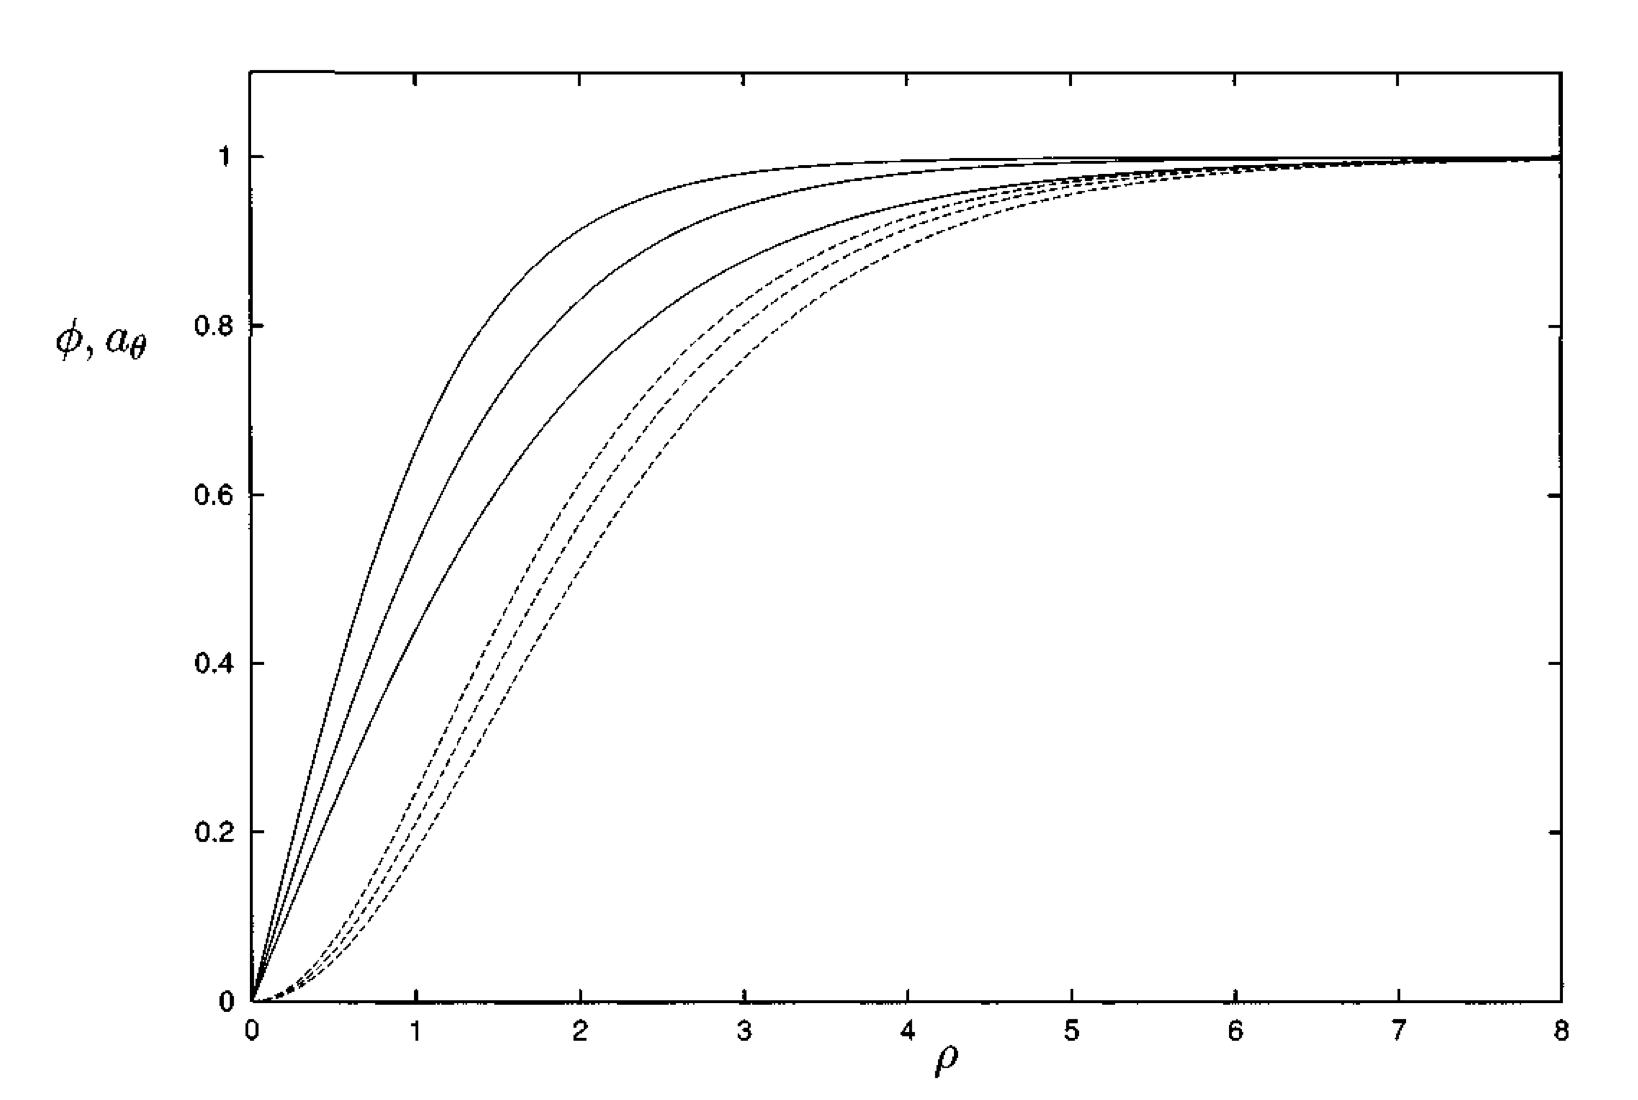
\includegraphics[width=0.5\linewidth]{fig/fig2.png}
            \caption{Figure taken from [Manton \& Sutcliffe]. The profile functions $\phi(\rho)$ (solid curves) and $a_\theta(\rho)$ (dashed curves) for the $N = 1$ vortex with $\lambda = 0.5,1.0,2.0$. The curves move to the left with increasing $\lambda$. Here, $\phi(\rho) \equiv h(r)$ and $a_\theta(\rho) \equiv f(r)$ in our context.}
        \end{figure}
    \end{ex}
    

    \subsection{Vortices at Critical Coupling, and the Bogomolny Equations}

    \lec{7} Here we choose $\lambda = 1$. 

    \begin{thm}
        The energy of $\lambda = 1$ vortices with vortex number $N$ (assumed wlog to be $\geq 0$) is bounded from below 
        \begin{equation}
            E \geq \pi N 
        \end{equation}
        with equality if the Bogomolny equations 
        \begin{align}
            (D_1 + \mathrm{i} D_2) \phi = 0 \label{eq:vtx-b1}\\
            B = \frac{1}{2} \left( 1 - \abs{\phi}^2 \right)\label{eq:vtx-b2}
        \end{align}
        hold.
    \end{thm}
    \begin{proof}
        Rewrite (\ref{eq:vtx-E}) as 
        \begin{equation}
            \begin{split}
                E & = \underbrace{\frac{1}{2} \int_{\mathbb{R}^2} \left( \left( B - \frac{1}{2} \left( 1 - \abs{\phi}^2 \right) \right)^2 + \overline{(D_1 + \mathrm{i} D_2)\phi} (D_1 + \mathrm{i} D_2) \phi \right) \dd{x^1} \dd{x^2}}_{E_1}\\
                & \qquad + \underbrace{\frac{1}{2} \int_{\mathbb{R}^2} \left\{ B \left( 1 - \abs{\phi}^2 \right) - \mathrm{i}\left( \overline{D_1 \phi} D_2 \phi - D_1 \phi \overline{D_2 \phi}\right) \right\} \dd{x^1} \dd{x^2}}_{E_2}
            \end{split}
        \end{equation}
        where 
        \begin{equation}
            E_2 = \frac{1}{2} \int_{\mathbb{R}^2} F + \underbrace{\int_{\mathbb{R}^2} \left( \cdots \right) \dd{x^1} \dd{x^2}}_{=0 \text{ by Stokes' thm}}
        \end{equation}
        (to show it, use the Leibniz rule, and $[D_1, D_2] \phi = -\mathrm{i} B \phi$). Then
        \begin{equation}
            E = {\underbrace{E_1}_{\geq 0}} + \pi N = \pi N \quad \text{if} \quad E_1 = 0
        \end{equation}
        where we have (\ref{eq:vtx-b1}) and (\ref{eq:vtx-b2}).
    \end{proof}

    Any solution to (\ref{eq:vtx-b1}) and (\ref{eq:vtx-b2}) also solves the full field equation (\ref{}).

    The Bogomolny equations are not integrable. They are however reducible to a single 2nd-order scalar PDE (the Taubes equation). 

    Write $\phi = e^{\frac{u}{2} + \mathrm{i} \chi}$ where $u, \chi$ are real-valued, with $u$ gauge invariant.

    \begin{equation}
        \begin{split}
            (\ref{eq:vtx-b1}) \quad \implies \quad \left[ (\partial_1 - \mathrm{i} A_1) + \mathrm{i}(\partial_2 - \mathrm{i} A_2) \right] e^{\frac{u}{2} + \mathrm{i} \chi} & = 0\\
            e^{u/2 + \mathrm{i} \chi} \left( \frac{1}{2} \partial_1 u + \mathrm{i} \partial_1 \chi - \mathrm{i} A_1 + \frac{\mathrm{i}}{2} \partial_2 u - \partial_2 \chi + A_2 \right) & = 0
        \end{split}
    \end{equation}
    matching the real and imaginary parts, we have 
    \begin{equation}
        A_1 = \partial_1 \chi + \frac{1}{2} \partial_2 u, \qquad A_2 = \partial_2 \chi - \frac{1}{2} \partial_1 u 
    \end{equation}
    and in terms of a differential form, we have 
    \begin{equation}
        A = \dd{\chi} + \frac{1}{2} \left( \partial_2 u \dd{x^1} - \partial_1 u \dd{x^2} \right).
    \end{equation}
    Now that (\ref{eq:vtx-b1}) has been solved, we look at 
    \begin{equation}
        (\ref{eq:vtx-b2}) \quad \implies \quad B = \frac{1}{2} \left( 1 - \abs{\phi}^2 \right).
    \end{equation}
    Firstly, 
    \begin{equation}
        F = \dd{A} = - \frac{1}{2} \left( \partial_1^2 + \partial_2^2 \right) u \dd{x^1} \wedge \dd{x^2}
    \end{equation}
    so we have 
    \begin{equation}
        B = - \frac{1}{2} \Delta u 
    \end{equation}
    where $\Delta$ is the Laplacian. Finally, we obtain 
    \begin{equation}
        \boxed{\Delta u = e^u - 1} \label{eq:Taubes}
    \end{equation}
    the Taubes equation.

    (\ref{eq:Taubes}) is valued outside the zeros of $\phi$. Say that $\phi$ has a zero of order-$k$ at some $Z$ [set $z = x+\mathrm{i}y$, $\underbrace{Z = X + \mathrm{i} Y}_{\text{fixed}}$], then 
    \begin{equation}
        \abs{\phi}^2 \sim \text{const.} \abs{z - Z}^{2k}
    \end{equation}
    so near $Z$, $u$ has the form 
    \begin{equation}
        u = 2k \ln \left( |z - Z| \right) + \underbrace{\cdots}_{\text{regular}}.
    \end{equation}
    
    Set boundary conditions $\abs{\phi}\to 1$ at $\infty$ so $u \to 0$ as $|z| \to \infty$.

    \begin{thm}[Taubes]
        A vortex is specified uniquely by a set of $N$ points on $\mathbb{R}^2$, and the multiplicities of zeroes. If all multiplicities are $1$ (generic), then the \textbf{moduli space} of solutions (modulo gauge) to (\ref{eq:vtx-b1},\ref{eq:Taubes}) is $2N$-dimensional.
    \end{thm}

    \begin{ex}
        $N=1$. Choose the location of the vortex to be the origin of $\mathbb{R}^2$ in plane polars. (\ref{eq:Taubes}) gives 
        \begin{equation}
            u'' + \frac{1}{r} u' = e^u - 1
        \end{equation}
        where $u = u(r)$ subject to 
        \begin{equation}
            u(r) = \begin{cases}
                2 \ln(r) + u_0 + \underbrace{u_1}_{=0} r + u_2 r^2 + \cdots & \text{near }0\\
                0 & \text{as }r \to \infty.
            \end{cases}
        \end{equation}
        Near $\infty$, 
        \begin{equation}
            e^u \sim 1 + u + \mathcal{O}(u^2)
        \end{equation}
        where the equation becomes 
        \begin{equation}
            u'' + \frac{1}{r} u' = u
        \end{equation}
        which is the \emph{modified Bessel equation} of order 0. We only keep the solution 
        \begin{equation}
            K_0(r) \sim \sqrt{\frac{\pi}{2 r}} e^{-r} \quad \text{as} \quad r\to \infty 
        \end{equation}
        as the other solution $J_0(r)$ has the wrong asymptotics. So $u \sim c K_0(r)$ for $r \to \infty$ and some constant $c$. Numerically, 
        \begin{equation}
            c \simeq 3.41.
        \end{equation}
    \end{ex}

    \subsection{Vortices on Curved Surfaces ($\lambda = 1$)}
    Spacetime $2+1$ dimensional, $\mathbb{R} \times \Sigma$ with the metric $\dd{t^2} - g$. $(\Sigma, g)$ is a curved surface with metric 
    \begin{equation}
        g = \Omega \left( \dd{x^2} + \dd{y^2} \right) = \Omega(z,\bar z) \dd{z} \dd{\bar z}
    \end{equation}
    with $z = x+\mathrm{i} y$ is the \emph{isothermal coordinate}. 

    Now 
    \begin{equation}
        E[\phi, A] = \frac{1}{2} \int_\Sigma \left\{ \frac{B^2}{\Omega^2} + \frac{1}{\Omega} \left( \overline{D_1 \phi} D_1 \phi + \overline{D_2 \phi} D_2 \phi + \frac{1}{4}\left( 1 - \abs{\phi}^2 \right)\right) \right\} \Omega \dd{x^1} \dd{x^2}
    \end{equation}
    where 
    \begin{equation}
        F = B \dd{x^1} \wedge \dd{x^2}, \quad \epsilon = \Omega \dd{x^1} \wedge \dd{x^2}.
    \end{equation}

    The Bogomolny equations read 
    \begin{align}
        & D_{\bar z} \phi = 0\\
        & B = \frac{\Omega}{2} \left( 1 - \abs{\phi}^2 \right)
    \end{align}
    and recall that 
    \begin{equation}
        \pdv{\bar z} = \frac{1}{2}\left( \pdv{x^1} + \mathrm{i} \pdv{x^2} \right)
    \end{equation}
    so 
    \begin{equation}
        D_{\bar z} = \frac{1}{2} \left( D_1 + \mathrm{i} D_2 \right).
    \end{equation}

    \lec{8} 

    Assume $\Sigma$ is compact, and integrate the Bogomolny equation for $B$ over $\Sigma$, we get
    \begin{equation}
        \int_\Sigma B \dd{x} \wedge \dd{y} = \int_\Sigma \left( \frac{1}{2} \Omega - \frac{1}{2} \abs{\phi}^2 \Omega \right) \dd{x} \wedge \dd{y}.
    \end{equation}

    Recall that 
    \begin{equation}
        \frac{1}{2 \pi} \int_{\mathbb{R}^2} F = N = \text{vortex number},
    \end{equation}
    and it is still true that 
    \begin{equation}
        \frac{1}{2 \pi} \int_\Sigma F = \text{integer }N = c_1 = \text{1st Chern number}.
    \end{equation}
    Now 
    \begin{equation}
        2 \pi N = \underbrace{\frac{1}{2} \int_\Sigma \Omega \dd{x} \wedge \dd{y}}_{\text{Area}(\Sigma)} - \frac{1}{2} \int_\Sigma \abs{\phi}^2 \Omega \dd{x} \wedge \dd{y}
    \end{equation}
    so in the compact case we have 
    \begin{equation}
        \boxed{\text{Area}(\Sigma) \geq 4 \pi N}
    \end{equation}
    which is the \emph{Bradlow bound}.

    Physicists' explanation: vortices are solitons of finite, non-zero size. The surface must be large enough for $N$ of them to fit in.

    Recall that $\phi = e^{u/2 + \mathrm{i} \chi}$. The Taubes equation is 
    \begin{equation}
        \Delta_0 u = \Omega (e^u - 1)
    \end{equation}
    with derivation as for $\mathbb{R}^2$. We have 
    \begin{equation}
        \Delta_0 = \left( \pdv{x} \right)^2 + \left( \pdv{y} \right)^2 = 4 \pdv{}{z}{\bar z}
    \end{equation}
    is the Laplacian of $\dd{z} \dd{\bar z}$.

    The maximum principle applied to $\Delta_0$: 
    \begin{enumerate}[1)]
        \item Assume $\Sigma$ is compact, then $u$ is bounded from above by $u_\text{max}$ and it attains the bound. Hessian of $u$ must be non-positive at $u_\text{max}$. Its trace is $\Delta u|_{u_\text{max}}$ so $\Delta u|_{u_\text{max}} \leq 0$. So, by Taubes equation, \begin{equation}
            \Omega (e^{u_\text{max}} - 1) \leq 0
        \end{equation} 
        so $u_\text{max} \leq 0$ hence 
        \begin{equation}
            \boxed{u \leq 0 \text{ on }\Sigma}.
        \end{equation}
        \item If $\Sigma$ is non-compact (e.g., $\mathbb{R}^2$), then $u \to -\infty$ at vortex positions, and $u \to 0$ at $\infty$ (for $\mathbb{R}^2$) or at $\partial \Sigma$. So $u \leq 0$ on $\Sigma$, or otherwise it would have to have a maximum $u_\text{max}$ with $u_\text{max} \geq 0$, which contradicts the Taubes equation. 
    \end{enumerate}

    \begin{ex}[Hyperbolic vortices]
        Take $\Sigma$ to be a Poincar\'e disc 
        \begin{equation}
            \Sigma = \mathbb{D} = \left\{ z\in \mathbb{C}, |z| < 1 \right\}
        \end{equation}
        with Gaussian curvature $-1/2$. The metric on $\Sigma$ is 
        \begin{equation}
            g = \frac{8}{\left( 1 - \abs{z}^2 \right)^2} \dd{z} \otimes \dd{\bar z}.
        \end{equation}
        \begin{figure}[H]
            \centering
            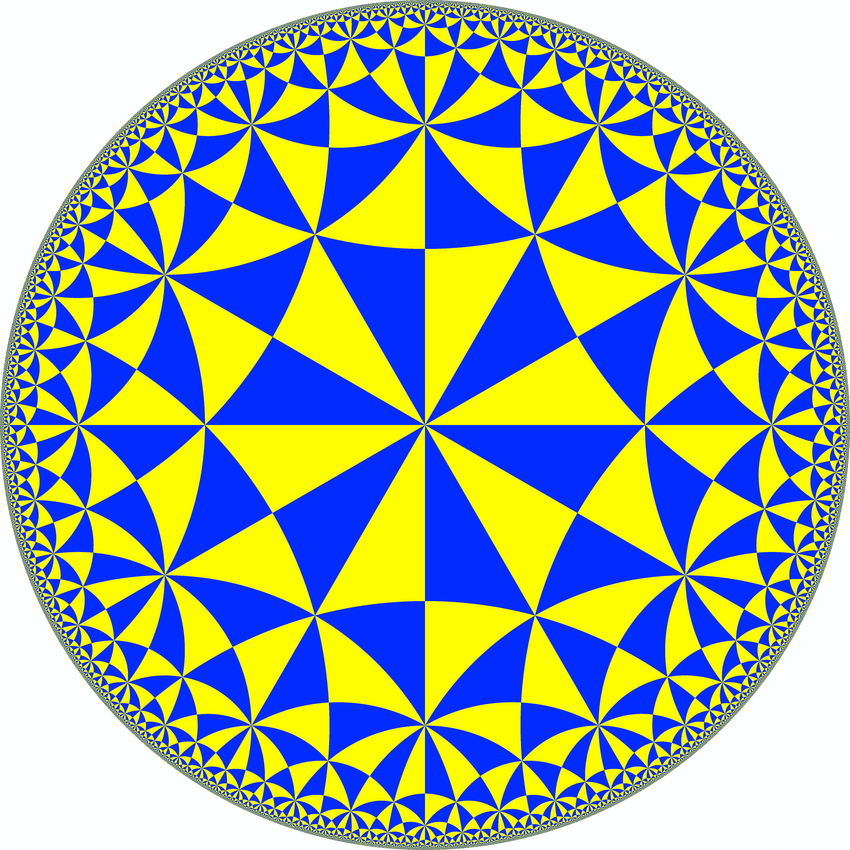
\includegraphics[width=0.25\linewidth]{fig/poincare.png}
        \end{figure}
        Witten (around 1977) found that the Bogomolny equations on $\mathbb{D}$ linearise and reduce to the Liouville's equation.

        Start with the Taubes equation 
        \begin{equation}
            \Delta_0 u = \Omega (e^u-1), \quad \Omega = \frac{8}{\left( 1 - \abs{z}^2 \right)^2}
        \end{equation}
        and set $u = \sigma - \ln \Omega$ to get 
        \begin{equation}
            \begin{split}
                \Delta_0 \sigma - \Delta_0 \ln \Omega & = \Omega \left( e^\sigma \Omega^{-1} - 1 \right)\\
                \Delta_0 \sigma - e^{\sigma} & = \underbrace{\Delta_0 \ln \Omega - \Omega}_{0}
            \end{split}
        \end{equation}
        So the Taubes equation reduces to the Liouville equation
        \begin{equation}
            \boxed{\Delta_0 \sigma = e^\sigma}
        \end{equation}
        which is completely solvable. So we can compute $\sigma \to u \to \abs{\phi}^2$. Up to gauge, we can find 
        \begin{equation}
            \phi = \frac{1 - \abs{z}^2}{1 - \abs{f}^2} \dv{f}{z}
        \end{equation}
        where $f = f(z)$, i.e., $\bar \partial f = 0$ and $|f| < 1$.

        Take $f$ to be the Blaschke function $|f| < 1$ 
        \begin{equation}
            f(z) = \prod_{k=1}^{N} \frac{c_k - z}{1 - \bar c_k z}
        \end{equation}
        where $c_1, \cdots c_N$ are constants with $|c_i| < 1$.
    \end{ex}

    \begin{ex}[Sinh-Gordon vortex]
        Take $\Omega = e^{-u/2}$ in the Taubes equation, then 
        \begin{equation}
            \Delta_0 u = e^{-u/2}(e^{u} - 1) = 2\sinh(u/2)
        \end{equation}
        and we obtain the \emph{Sinh-Gordon} equation
        \begin{equation}
            \boxed{\Delta_0 \left( \frac{u}{2} \right) = \sinh(\frac{u}{2})}
        \end{equation}
        which is integrable.

        Now $g = e^{-u/2} \dd{z} \otimes \dd{\bar z}$, so $(\Sigma, g)$ \emph{is} a vortex.
    \end{ex} 
    \newpage

    \section{Non-Abelian Gauge Theory and Instantons}
    \subsection{Hodge Duality}
    \lec{9} Start with $(\mathbb{R}^n, \eta)$ where $\eta = \dd{\vb x^2} - \dd{\vb t^2}$ with signature of $\eta$ is $(n-t,t)$, i.e.,
    \begin{equation}
        \eta = \mqty(\dmat{1,\ddots,1,-1,\ddots,-1})
    \end{equation}
    We choose coordinates $x^a = (\vb x, \vb t)$, $a=1,\cdots,n$.
    
    We pick an orientation 
    \begin{equation}
        \text{Vol} = \frac{1}{n!} \epsilon_{a_1 \cdots a_n} \dd{x^{a_1}}\wedge \cdots \wedge \dd{x^{a_n}}.
    \end{equation}
    
    For $p$-forms $\lambda, \mu \in \Lambda^p(\mathbb{R}^n)$ we have 
    \begin{equation}
        \lambda = \frac{1}{p!} \lambda_{a_1 \cdots a_p} \dd{x^{a_1}}\wedge \cdots \wedge \dd{x^{a_p}}, \quad \mu = \frac{1}{p!} \mu_{a_1 \cdots a_p} \dd{x^{a_1}}\wedge \cdots \wedge \dd{x^{a_p}}
    \end{equation}
    and the $\eta$-induced inner product on $\Lambda^p$ is defined as 
    \begin{equation}
        (\lambda, \mu) = \frac{1}{p!} \lambda_{a_1 \cdots a_p} \mu^{a_1 \cdots a_p} = (\mu, \lambda).
    \end{equation}

    We define a map $*:\Lambda^p \to \Lambda^{n-p}$, $\lambda \mapsto *\lambda \in \Lambda^{n-p}$ such that 
    \begin{equation}
        \mu \wedge * \lambda = (\mu, \lambda) \text{Vol}
    \end{equation}
    or, in coordinates 
    \begin{equation}
        (* \lambda)^{a_1\cdots a_q} = \frac{1}{p!} \epsilon\indices{^{a_1 \cdots a_q}_{b_1 \cdots b_p}} \lambda^{b_1 \cdots b_p}
    \end{equation}
    where $q = n-p$.

    We get 
    \begin{equation}
        *{*\lambda} = (-1)^t (-1)^{p(n-p)} \lambda
    \end{equation}

    \begin{ex}
        Consider Maxwell equations: $n=4,t=1,p=2$ here. 
        \begin{equation}
            \eta = \dd{x^2} + \dd{y^2} + \dd{z^2} - \dd{t^2}
        \end{equation}
        and 
        \begin{equation}
            \norm{\dd{y}\wedge \dd{z}}^2 = 1, \quad \norm{\dd{t}\wedge \dd{x}}^2 = -1
        \end{equation}
        we have 
        \begin{equation}
            *(\dd{t}\wedge \dd{x}) = \dd y \wedge \dd z, \quad *(\dd y \wedge \dd z) = - \dd t \wedge \dd x
        \end{equation}
        etc. On $2$-forms, $*^2 = - \text{id}$. 

        For $F \in \Lambda^2(\mathbb{R}^{3,1})$ with orientation $\epsilon_{0ijk} = \epsilon_{ijk}$, then 
        \begin{equation}
            F = F_{0i} \dd {t} \wedge \dd {x^i} + \frac{1}{2} F_{ij} \dd {x^i} \wedge \dd {x^j} = - E_i \dd{t} \wedge \dd{x^i} + \frac{1}{2} \epsilon_{ijk} B_k \dd{x^i} \wedge \dd{x^j}
        \end{equation}
        where $(\vb E, \vb B)$ are the electric + magnetic fields. 
        
        We also have 
        \begin{equation}
            * F = B_k \dd{t}\wedge \dd{x^k} + \frac{1}{2} \epsilon_{ijk} E_i \dd{x^j} \wedge \dd{x^k}
        \end{equation}
        so we identify 
        \begin{equation}
            *(\vb E, \vb B) = (- \vb B, \vb E).
        \end{equation}

        For the gauge potential $A\in \Lambda^1$, 
        \begin{equation}
            A = - \phi \dd{t} + A_i \dd{x^i}
        \end{equation}
        so the Maxwell field is 
        \begin{equation}
            F = \dd{A} = -\pdv{\phi}{x^i} \dd{x^i} \wedge \dd{t} + \pdv{A_i}{t} \dd{t} \wedge \dd{x^i} + \partial_{[i} A_{j]} \dd{x^i} \wedge \dd{x^j}
        \end{equation}
        to get 
        \begin{equation}
            \vb E = - \grad \phi - \dot{\vb A}, \quad \vb B = \curl \vb A
        \end{equation}
        and the Maxwell's equations are fully described by the Bianchi identity
        \begin{equation}
            \dd{F} = 0
        \end{equation}
        and 
        \begin{equation}
            \dd{* F} = 0.
        \end{equation}
    \end{ex}

    \begin{ex}[Self Duality]
        Take $p=2, n=4, t=0$, $\eta_{ab} = \delta_{ab}$ (Euclidean metric). Here, on $\Lambda^2$, $*^2 = \text{id}$. Consider $F \in \Lambda^2$, we can write 
        \begin{equation}
            F = \underbrace{\frac{1}{2} (F + *F)}_{F_+} + \underbrace{\frac{1}{2} (F - *F)}_{F_-} \label{eq:sd-asd}
        \end{equation}
        and 
        \begin{equation}
            * F_+ = \frac{1}{2} (* F + *{*F}) = F_+, \quad * F_- = - F_-
        \end{equation}
        so we call $F_+$ self-dual (SD), and $F_-$ anti-self-dual (ASD). Eq \eqref{eq:sd-asd} gives a decomposition 
        \begin{equation}
            \underbrace{\Lambda^2(\mathbb{R}^4)}_{\text{dim 6}} = \underbrace{\Lambda^2_+}_{\text{dim 3}} \oplus \underbrace{\Lambda^2_-}_{\text{dim 3}}
        \end{equation}
        where $\Lambda^2_+$ are SD 2 forms, $\Lambda^2_-$ are ASD 2 forms. In fancier notations, this is a realisation of 
        \begin{equation}
            \mathfrak{so}(4) = \mathfrak{so}(3) \oplus \mathfrak{so}(3)
        \end{equation}
        (unique to dimension 4).

        The Bianchi identity is $\dd{F} = 0$ (if $F = \dd{A}$). If $*F = F$, then 
        \begin{equation}
            \dd{*F} = \dd{F} = 0
        \end{equation}
        then the Maxwell's equation holds as a consequence of the Bianchi identity. 
    \end{ex}
    
    \subsection{Yang-Mills Equations}
    Take $(\mathbb{R}^n, \eta, \text{Vol})$ and $\mathfrak{g}$ a Lie algebra of a Lie group $G$. 

    Let $T_\alpha$, $\alpha = 1, \cdots, \dim(G)$ be the basis of $\mathfrak{g}$ and they satisfy 
    \begin{equation}
        [T_\alpha, T_\beta] = c_{\alpha \beta \gamma} T_\gamma
    \end{equation} 
    where $c_{\alpha \beta \gamma}$ are the \emph{structure constants}.

    Now let $A$ be a $\mathfrak{g}$-valued 1-form (gauge potential), so 
    \begin{equation}
        A = A_a \dd{x^a} = A\indices{_a^\alpha} T_\alpha \dd{x^a}
    \end{equation}
    so the gauge field is 
    \begin{equation}
        F = \dd{A} + A \wedge A = \frac{1}{2} F_{ab} \dd{x^a} \wedge \dd{x^b}
    \end{equation}
    with
    \begin{equation}
        F_{ab} = \partial_a A_b - \partial_b A_a + [A_a, A_b] = [D_a, D_b]
    \end{equation}
    where 
    \begin{equation}
        D = \dd{} + A
    \end{equation}
    is a covariant derivative. We further obtain 
    \begin{equation}
        D F \equiv \dd{F} + [A,F] = 0,
    \end{equation}
    which is the covariant Bianchi identity.
    \begin{proof}
        \begin{equation}
            D F = \dd[2]{A} + \dd{A} \wedge A - A \wedge \dd{A} + A \wedge (\dd{A} + A \wedge A) - (\dd{A} + A \wedge A) \wedge A = 0
        \end{equation}
    \end{proof}
    
    In the non-abelian case, a gauge transformation is 
    \begin{equation}
        (A,F) \sim (A',F')
    \end{equation}
    where 
    \begin{equation}
        A' = g A g^{-1} - (\dd{g}) g^{-1}, \quad F' = g F g^{-1}
    \end{equation}
    where $g = g(x^a) \in G$.

    For example, in the case $G = \SU(2)$, $\det g = 1$ so $g^{\dagger} g = 1$. The Lie algebra $\mathfrak{su}(2)$ is a Lie algebra of traceless anti-Hermitian matrices, and it has commutation relations 
    \begin{equation}
        [T_\alpha, T_\beta] = - \epsilon_{\alpha \beta \gamma} T_\gamma
    \end{equation}
    and 
    \begin{equation}
        \Tr(T_\alpha) = 0, \quad \Tr(T_\alpha T_\beta) = -\frac{1}{2} \delta_{\alpha \beta}.
    \end{equation}

    \begin{nt}
        Notice 
        \begin{equation}
           - \Tr(F \wedge *F) = \frac{1}{2} F_{ab} F^{ab} 
        \end{equation}
        so we choose the Yang-Mills action as 
        \begin{equation}
            S[A] = - \int_{\mathbb{R}^n} \Tr(F \wedge * F). \label{eq:YM-action}
        \end{equation}
    \end{nt}

    \begin{exer}
        Show that the Euler-Lagrange equation for $S$ reads 
        \begin{equation}
            \boxed{D {*F} = 0} \label{eq:YM-eom}
        \end{equation}
        which is the Yang-Mill equation.
    \end{exer}

    \subsection{Yang-Mills Instantons}\lec{10} 
    Here, we work in $\mathbb{R}^4$ and Euclidean metric $\eta_{ab} = \delta_{ab}$. 
    \begin{defi}[Instanton]
        Instantons are solutions to \eqref{eq:YM-eom} on $(\mathbb{R}^4, \eta)$ with Euclidean signature whose action is finite. 
    \end{defi}

    For the action to be finite, we take boundary conditions
    \begin{equation}
        \begin{split}
            F_{ab}(x) & \sim \mathcal{O}\left( \frac{1}{r^3} \right) \quad \text{as} \quad r \to \infty, \quad r^2 \equiv \delta_{ab} x^a x^b\\
            A_a(x) & \sim \mathcal{O}\left( \frac{1}{r^2} \right) - (\partial_a g) g^{-1} \quad \text{up to gauge}
        \end{split}
    \end{equation}
    where $g$ is only required to be defined asymptotically for $r \to \infty$.

    So $g: S^3_{\infty} \to \SU(2) \simeq S^3$ where $S^3_{\infty}$ is the 3-sphere at $r=\infty$ which can be identified as $\partial \mathbb{R}^4$. It is partially characterised by its topological degree \eqref{eq:su-2}. 

    \begin{rmk}
        Consider a gauge theory on $\mathbb{R}^n$. We define the Chern form through 
        \begin{equation}
            C(F) = \det(\1 + \frac{\mathrm{i}}{2 \pi} F) = 1 + C_1(F) + C_2(F) + \cdots 
        \end{equation}
        where $C_p$ of $F$ is a $2p$-form and is called the $p^{\text{th}}$ Chern form.

        This is a polynomial in traces of powers of $F$: 
        \begin{equation}
            \begin{split}
                C_1(F) & = \frac{\mathrm{i}}{2 \pi} \Tr(F) \begin{cases}
                    = 0, & \mathfrak{g} = \mathfrak{su}(2),\\
                    \neq 0, & \mathfrak{g} = \mathfrak{u}(1).
                \end{cases}\\
                C_2(F) & = \frac{1}{8 \pi^2}\bigg( \Tr(F \wedge F) - \underbrace{\Tr(F) \wedge \Tr(F)}_{=0 \text{ for }\mathfrak{su}(2)} \bigg)\\
                C_3(F) & = \cdots
            \end{split}
        \end{equation}

        All Chern forms are gauge invariant 
        \begin{equation}
            C(g F g^{-1}) = \det(\1 + \frac{\mathrm{i}}{2 \pi} g F g^{-1}) = C(F)
        \end{equation}
        and closed (by Bianchi identity).

        Check this for $C_2(F)$: 
        \begin{equation}
            \begin{split}
                \dd{C_2} & = \frac{1}{4 \pi^2} \Tr(\dd{F} \wedge F)\\
                & = \frac{1}{4 \pi^2} \Tr(D F \wedge F - A \wedge F \wedge F + F \wedge A \wedge F) = 0
            \end{split}
        \end{equation}
        by $DF = \dd{F} + [A,F]$, the Bianchi identity, and trace permutations.

        On $\mathbb{R}^n$, if $\dd{C_2} = 0$, then $C_2 = \dd{Y_3}$ for some $3$-form $Y_3$, the \emph{Chern-Simons} form. We can calculate (as an exercise) 
        \begin{equation}
            Y_3 = \frac{1}{8 \pi^2} \Tr(A \wedge \dd{A} + \frac{2}{3} A \wedge A \wedge A).
        \end{equation}
    \end{rmk} 

    Integrals of maximal Chern forms are integers: the \emph{Chern numbers}.

    Go back to $n=4$, 
    \begin{equation}
        c_2 = \int_{\mathbb{R}^4} C_2(F) = \int_{\mathbb{R}^4} \dd{Y_3} = \int_{S^3_{\infty}} Y_3 = \frac{1}{8 \pi^2}\int_{S^3_{\infty}} \Tr(A \wedge F - \frac{1}{3} A \wedge A \wedge A)
    \end{equation}
    where we used $F = \dd{A} + A \wedge A$. Use the boundary conditions at $\infty$, $F=0$ and $A = - (\dd{g_{\infty}}) g_{\infty}^{-1}$ where $g_{\infty} : S^3_\infty \to \SU(2) \simeq S^3$, so 
    \begin{equation}
        c_2 = \frac{1}{24 \pi^2} \int_{S^3_\infty} \Tr([\dd{g_\infty} \cdot g_{\infty}^{-1}]^3) = \deg(g_\infty) \in \mathbb{Z}
    \end{equation} 
    by \eqref{eq:su-2}.

    Assume (by choosing the orientation) that $c_2 \geq 0$. Then 
    \begin{thm}
        The Yang-Mills action of instantons is bounded from below by $S[A] \geq 8 \pi^2 c_2$ with equality if anti-self-dual Yang-Mills (ASDYM) equations 
        \begin{equation}
            *F = - F, \label{eq:ASDYM}
        \end{equation}
        i.e.,
        \begin{equation}
            F_{12} = - F_{34}, \quad F_{13} = - F_{42}, \quad F_{14} = - F_{23} 
        \end{equation}
        hold.
    \end{thm}
    \begin{proof}
        Note that (exercise) $F \wedge F = *F \wedge *F$. So 
        \begin{equation}
            \begin{split}
                S[A] & = -\int_{\mathbb{R}^4} \Tr(F \wedge *F)\\
                & = - \frac{1}{2} \int_{\mathbb{R}^4} \underbrace{\Tr[(F + *F) \wedge *(F + *F)]}_{\leq 0} + \underbrace{\int_{\mathbb{R}^4} \Tr(F \wedge F)}_{8 \pi^2 c_2} \geq 8 \pi^2 c_2 
            \end{split}
        \end{equation}
        with equality holds at $F + *F = 0$.
    \end{proof}
    \begin{rmk}
        ~ \begin{itemize}
            \item \eqref{eq:ASDYM} are a system of 1st order PDEs. If $A$ satisfies it, then \begin{equation}
                D {*F} = - D F = 0
            \end{equation}
            so \eqref{eq:YM-eom} holds;
            \item If $c_2 \leq 0$ (or change orientation), then ASDYM becomes SDYM $F = *F$;
            \item $k = -c_2$ is the instanton number.
        \end{itemize}
    \end{rmk}
    \subsection{Zero Curvature Representation for ASDYM}
    \lec{11} ASDYM is a master integrable system (Richard Ward et al.~late 80' and early 90'). Most lower dimensional integrable soliton equations (like KdV, Sine-Gordon, NLS, ...) arise as symmetry reductions of \eqref{eq:ASDYM}. 
    
    \eqref{eq:ASDYM} arises as a compatibility condition for an over-determined system of linear PDEs, i.e., there is a Lax pair. Let's find it. 

    Use complexified Minkowski space $M_{\mathbb{C}} = \mathbb{C}^4$ with 
    \begin{equation}
        \eta = 2 (\dd{z} \dd{\tilde z} - \dd{w} \dd{\tilde w}), \quad \text{vol} = \dd{w} \wedge \dd{\tilde w} \wedge \dd{z} \wedge \dd{\tilde z}
    \end{equation}
    where $(w, \tilde w, z, \tilde z)$ is the complex (double null) coordinates on $\mathbb{C}^4$.

    The real slices of complexified Minkowski $\mathbb{C}^4$ are
    \begin{enumerate}[1)]
        \item Euclidean $({+}{+}{+}{+})$\footnote{Signatures only make sense for real manifolds.} \begin{equation}
            z = \frac{x^1 + \mathrm{i} x^2}{\sqrt{2}}, \quad \tilde z = \bar z, \quad w = \frac{x^3 + \mathrm{i} x^4}{\sqrt{2}}, \quad \tilde w = - \bar w;
        \end{equation}
        \item Minkowski $({+}{+}{+}{-})$ \begin{equation}
            z = \frac{x^1 + \mathrm{i} x^2}{\sqrt{2}}, \quad \tilde z = \bar z, \quad w = \frac{x^4 + x^3}{\sqrt{2}}, \quad \tilde w = \frac{x^4 - x^3}{\sqrt{2}};
        \end{equation}
        \item Neutral/ultrahyperbolic $({+}{+}{-}{-})$, $w, \tilde w, z, \tilde z$ are all real.
    \end{enumerate}

    Basis of SD 2-forms is 
    \begin{equation}
        \omega^1 = \dd{w} \wedge \dd{z}, \quad \omega^2 = \dd{w} \wedge \dd{\tilde w} - \dd{z} \wedge \dd{\tilde z}, \quad \omega^3 = \dd{\tilde w} \wedge \dd{\tilde z}.
    \end{equation}

    A two form $F$ is ASD if \eqref{eq:ASDYM} holds. Equivalently (exercise) if 
    \begin{equation}
        F \wedge \omega^j = 0, \quad j = 1,2,3.
    \end{equation}
    \eqref{eq:ASDYM} becomes 
    \begin{equation}
        F_{wz} = 0, \quad F_{w \tilde w} - F_{z \tilde z} = 0, \quad F_{\tilde w \tilde z} = 0 \label{eq:complex-ASD}.
    \end{equation}
    and we find
    \begin{equation}
        [D_w, D_z] = 0.
    \end{equation}


    \begin{aside}[What are ``compatibility conditions''?]
    Consider an example n $\mathbb{R}^2$: $A_x(x,y)$, $A_y(x,y)$ are two $2\times 2$ matrices. Consider an overdetermined linear PDE system 
    \begin{equation}
        \underbrace{\partial_x v + A_x v = 0}_{D_x v = 0}, \quad \underbrace{\partial_y v + A_y v = 0}_{D_y v = 0} \label{eq:2-vector-ex}
    \end{equation}
    where  
    \begin{equation}
        v = \mqty(v_1(x,y)\\v_2(x,y))
    \end{equation}
    is an unknown vector. 
    
    We start with 
    \begin{equation}
        \begin{split}
            0 & = \partial_y \partial_x v - \partial_x \partial_y v\\
            & = - \partial_y \left( A_x v \right) + \partial_x \left( A_y v \right)\\
            & = \left( - \partial_y A_x + A_x A_y + \partial_x A_y - A_y A_x \right) v\\
            & = F_{xy} v = [D_x, D_y] v.
        \end{split}
    \end{equation}
    So we need 
    \begin{equation}
        \boxed{F_{xy} = 0} \label{eq:zero-curvature-ex}
    \end{equation}
    if we want \eqref{eq:2-vector-ex} to be solvable for any initial data.

    \eqref{eq:zero-curvature-ex} is a zero curvature representation. Curvature $F$ of a ``connection'' $A_x \dd{x} + A_y \dd{y}$ has to vanish for \eqref{eq:2-vector-ex} to admit full solution space.

    Assume $F_{xy} = 0$. Combine two solutions of \eqref{eq:2-vector-ex} into a matrix fundamental solution $g$ obeying
    \begin{equation}
        \begin{split}
            0 & = D_x g = \partial_x g + A_x g\\
            0 & = D_y g = \partial_y g + A_y g
        \end{split}
    \end{equation}
    which gives  
    \begin{equation}
        A_x = - (\partial_x g) g^{-1}, \quad A_y = - (\partial_y g) g^{-1}.
    \end{equation}
    \end{aside}

    Back to ASDYM \eqref{eq:complex-ASD}, define a Lax pair with a parameter (spatial parameter) $\lambda \in \mathbb{CP}^1$ 
    \begin{equation}
        L = D_{\tilde z} - \lambda D_w, \quad M = D_{\tilde w} - \lambda D_z
    \end{equation}
    which gives an over-determined linear PDE 
    \begin{equation}
        L \Psi = 0,\quad M \Psi = 0
    \end{equation}
    where 
    \begin{equation}
        \Psi = \Psi(w,z,\tilde w, \tilde z; \lambda)
    \end{equation} 
    is a fundamental matrix solution. As before, the compatibility conditions are 
    \begin{equation}
        [L, M] = 0.
    \end{equation}
    
    We find 
    \begin{equation}
        \begin{split}
            0 & = [L,M]\\
            & = [D_{\tilde z} - \lambda D_w, D_{\tilde w} - \lambda D_z] \\
            & = \underbrace{[D_{\tilde z}, D_{\tilde w}]}_{F_{\tilde z \tilde w}} - \lambda \underbrace{\left( [D_w, D_{\tilde w}] - [D_z, D_{\tilde z}] \right)}_{F_{w \tilde w} - F_{z \tilde z}} + \lambda^2 \underbrace{[D_w, D_z]}_{F_{wz}}
        \end{split}
    \end{equation}
    which has to vanish for all $\lambda$. So $[L,M] = 0$ iff \eqref{eq:complex-ASD} hold. 

    If we know $\Psi(w,z,\tilde w, \tilde z; \lambda)$, then 
    \begin{equation}
        L \Psi = 0, M \Psi = 0 \quad \Leftrightarrow \quad \begin{cases}
            - (\partial_{\tilde z} - \lambda \partial_w) \Psi \cdot \Psi^{-1} = A_{\tilde z} - \lambda A_w\\
            - (\partial_{\tilde w} - \lambda \partial_z) \Psi \cdot \Psi^{-1} = A_{\tilde w} - \lambda A_z
        \end{cases}
    \end{equation}
    and we can read off $A$ from the above.

    Geometrical interpretation: 
    \begin{equation}
        l = \partial_{\tilde z} - \lambda \partial_w, \quad m = \partial_{\tilde w} - \lambda \partial_z
    \end{equation} 
    span totally null planes in $M_{\mathbb{C}}$. This is because 
    \begin{equation}
        \eta(l,l) = 0, \quad \eta(m,m) = 0, \quad \eta(l,m) = -2 \lambda + 2 \lambda = 0.
    \end{equation}

    Note 
    \begin{equation}
        \text{vol}(l,m,\cdot,\cdot) = \omega^1 + \lambda \omega^2 + \lambda^2 \omega^3
    \end{equation}
    which is self-dual for each $\lambda$. So $(l,m)$ span totally null, self-dual 2-planes. These are known as \emph{$\alpha$-planes}.

    \lec{12} Take 
    \begin{equation}
        A = A_w \dd{w} + A_{\tilde w} \dd{\tilde w} + A_z \dd{z} + A_{\tilde z} \dd{\tilde z} \in \Lambda^1(M_{\mathbb{C}}) \otimes \mathfrak{g}
    \end{equation}
    and 
    \begin{equation}
        L = l + l \lrcorner A, \quad M = m + m \lrcorner A
    \end{equation}
    which are directional covariant derivatives in directions of $(l,m)$. 
    \begin{equation}
        [L,M] = 0 \quad \Rightarrow \quad F(l,m) = 0.
    \end{equation}

    \begin{thm}
        ASDYM $*F = -F$ are equivalent to $F= \dd{A} + A \wedge A$ vanishing on all SD null planes (i.e., $\alpha$-planes).
    \end{thm}
    \begin{rmk}
        Space of $\alpha$-planes is called the \emph{twistor space}.
    \end{rmk}

    \begin{ex}[Symmetry reduction]
        Take $G = \SL(2,\mathbb{C})$. The Lie algebra is spanned by $T_\alpha$ such that 
        \begin{equation}
            [T_\alpha, T_\beta] = - \epsilon_{\alpha \beta \gamma} T_\gamma.
        \end{equation} 
        Take 
        \begin{equation}
            A_w = 2(\cos \phi T_1 + \sin \phi T_2), \quad A_{\tilde w} = 2 T_1, \quad A_z = (\partial_z \phi) T_3, \quad A_{\tilde z} = 0, \quad \phi = \phi(z,\tilde z).
        \end{equation}
        We calculate ASDYM as 
        \begin{equation}
            \pdv{\phi}{z}{\tilde z} + 4 \sin \phi = 0.
        \end{equation}
        If $z, \tilde z$ real (so ${+}{+}{-}{-}$ real slice of $M_{\mathbb{C}}$), this is the 1+1 dimensional Sine-Gordon equation.
    \end{ex}
    \newpage 
    \section{Lie Groups}
    \begin{defi}[Lie group]
        A \emph{Lie group} $G$ is a group, and also a smooth manifold such that the operations $g \mapsto g^{-1}$, $(g_1, g_2) \mapsto g_1 \cdot g_2$ are smooth maps between manifolds $G \to G$, $G \times G \to G$.
    \end{defi}
    \begin{ex}
        $G = \SU(2)$, $g \in G$ are complex matrices such that $g^{\dagger} g = \1$, $\det g = 1$. They can be parametrised by 
        \begin{equation}
            g = \mqty(a + \mathrm{i} b & c + \mathrm{i} d\\-(c - \mathrm{i} d) & a - \mathrm{i} b), \quad a^2 + b^2 + c^2 + d^2 = 1, \qquad S^3 \subset \mathbb{R}^4.
        \end{equation}
    \end{ex}

    \begin{defi}[Group action]
        A group $G$ acts on a manifold $M$ if there exists a map $\rho: G \times M \to M$ (we often write $\rho(g,m) = g(m)$), such that 
        \begin{equation}
            e(m) = m, \quad \forall m \in M, \qquad g_2(g_1(m)) = (g_2 \cdot g_1) m.
        \end{equation} 
    \end{defi}

    \begin{ex}
        Take $M = \mathbb{R}$, $G$ the 2D affine group with action on $M$ as 
        \begin{equation}
            \mathbb{R} \ni x \mapsto \tilde x = a x + b, \quad a \neq 0, b \in \mathbb{R},
        \end{equation}
        where $(a,b)$ can be taken as coordinates on $G$. Then, in matrix notation, elements of $G$ can be represented as 
        \begin{equation}
            \mqty(x\\1) \mapsto \mqty(\tilde x\\1) = \mqty(a & b\\0 & 1)\mqty(x\\1).
        \end{equation}
        The identity is $e = (1,0)$. 

        There are two 1-parameter subgroups: 
        \begin{equation}
            G_a : x \mapsto \tilde x = ax; \quad G_b : x \mapsto \tilde x = x + b.
        \end{equation}
        These are generated by 
        \begin{equation}
            \dv{\tilde x}{a} \pdv{\tilde x}\bigg|_{a=1} = x \pdv{x} =: V_a, \qquad \dv{\tilde x}{b} \pdv{\tilde x}\bigg|_{b=0} = \pdv{x} =: V_b.
        \end{equation}
        
        Taking the Lie bracket of these two vectors 
        \begin{equation}
            [V_b, V_a] = V_b,
        \end{equation}
        we find this is isomorphic to the 2-dimensional Lie algebra of affine group. 
    \end{ex}
    The above is the physicists' approach to Lie algebras from Lie groups. Below we will treat this from a more pure mathematicians' perspective.
    \newpage

    \subsection{Left Invariant Vector Fields}
    \begin{defi}[Lie algebra]
        $G$ is a Lie group. Define the Lie algebra $\mathfrak{g}$ of $G$ to be $T_e G$.
    \end{defi}
    \begin{defi}[Left translation]
        For each $g \in G$, define the left translation $L_g: G \to G$ by $L_g(h) = g \cdot h$.
    \end{defi}
    
    The tangent map at $e$ is the derivative of $L_g$
    \begin{equation}
        (L_g)_* : \underbrace{T_e G}_{\mathfrak{g}} \mapsto T_g G,
    \end{equation}
    i.e., to each element of $\mathfrak{g}$ this associates a vector field. 

    Pick a basis $\{T_\alpha\} = \{T_1, \cdots T_n\}$, $n = \dim G$ of $\mathfrak{g}$. There are $n$ vector fields $L_\alpha$ (left-invariant vector fields). 
    
    Define a bracket $[\cdot,\cdot]_\mathfrak{g} : \mathfrak{g} \times \mathfrak{g} \to \mathfrak{g}$ by 
    \begin{equation}
        (L_g)_* [V,W]_\mathfrak{g} = [(L_g)_*(V), (L_g)_*(W)], \quad \forall V,W \in \mathfrak{g}. \label{eq:lie-bracket}
    \end{equation}

    Understand the notation! RHS = Lie brackets of vector fields. \eqref{eq:lie-bracket} holds for all $g \in G$ and all $V,W \in \mathfrak{g}$ that it defines $[\cdot,\cdot]_\mathfrak{g}$ uniquely.

    Hence, $L_\alpha$ are left-invariant vector fields that 
    \begin{equation}
        [L_\alpha, L_\beta] = \sum_\gamma f\indices{_{\alpha \beta}^\gamma} L_\gamma
    \end{equation}
    where $f\indices{_{\alpha \beta}^\gamma}$ are the structure constants for $\mathfrak{g}$. 

    Left-invariant 1-forms $\sigma^\alpha$ are dual to $L_\beta$ via $L_\beta \lrcorner \sigma^\alpha = \delta^\alpha_\beta$.

    \begin{clm}
        \begin{equation}
            \dd{\sigma^\alpha} + \frac{1}{2} \sum_{\beta, \gamma} \sigma^\beta \wedge \sigma^\gamma = 0. \label{eq:MC}
        \end{equation}
    \end{clm}

    \lec{13} 
    \begin{proof}
    Assume that $G$ is a matrix Lie group, and define a Mouver-Cartan 1-form 
    \begin{equation}
        \rho = g^{-1} \dd{g}
    \end{equation}
    it has the following properties: 
    \begin{itemize}
        \item $\rho$ is left-invariant: if $g_0 \in G$ is a constant matrix then $(g_0 g)^{-1} \dd{(g_0 g)} = g^{-1} g_0^{-1} g_0 \dd{g} = g^{-1} \dd{g}$;
        \item $\rho$ is Lie algebra valued: take a curve $g(s)$ in $G$ then $g^{-1} g$ at $s+\epsilon$ is \begin{equation}
            g^{-1}(s) \left( g(s) + \epsilon \dv{g}{s}\bigg|_{\epsilon = 0} + \cdots \right) = \1 + \epsilon \underbrace{g^{-1} \dot g}_{\in \mathfrak{g}};
        \end{equation}
        \end{itemize}

        Calculate 
        \begin{equation}
            \dd{\rho} = \dd{(g^{-1} \dd{g})} = - g^{-1} \dd{g} g^{-1} \wedge \dd{g} = - \rho \wedge \rho
        \end{equation}
        so we have the Mouver-Cartan equation 
        \begin{equation}
            \boxed{\dd{\rho} + \rho \wedge \rho = 0}\,.
        \end{equation}
        $\rho$ is a $\mathfrak{g}$-valued 1-form
        \begin{equation}
            \rho = \sum_\alpha \sigma^\alpha \otimes T_\alpha
        \end{equation}
        where $T_\alpha$'s satisfy
        \begin{equation}
            [T_\alpha, T_\beta] = f\indices{_{\alpha \beta}^\gamma} T_\gamma.
        \end{equation}
        by using Mouver-Cartan equation, we have 
        \begin{equation}
            0 = \dd{\rho} + \rho \wedge \rho = \sum_\alpha \dd{\sigma^\alpha} \otimes T_\alpha + \underbrace{\sum_{\beta,\gamma} \sigma^\beta \wedge \sigma^\gamma \otimes T_{\beta} T_{\gamma}}_{\frac{1}{2} \sum_{\beta,\gamma} \sigma^\beta \wedge \sigma^\gamma [T_\beta, T_\gamma]} = \sum_\alpha \dd{\sigma^\alpha} \otimes T_\alpha + \frac{1}{2} \sum_{\beta,\gamma} \sigma^\beta \wedge \sigma^\gamma f\indices{_{\beta \gamma}^\alpha} \otimes T_\alpha 
        \end{equation}
        so we obtain finally
        \begin{equation}
            \dd{\sigma^\alpha} + \frac{1}{2} \sum_{\beta,\gamma} \sigma^\beta \wedge \sigma^\gamma f\indices{_{\beta \gamma}^\alpha} = 0.
        \end{equation}
    \end{proof}
    \begin{ex}
        Take $G$ the 3-dimensional Heisenberg group (Nil group). Any $g \in G$ takes the matrix form 
        \begin{equation}
            g = \mqty(1 & x & z\\0 & 1 & y\\0 & 0 & 1) = \1 + x T_1 + y T_2 + z T_3
        \end{equation}
        where 
        \begin{equation}
            T_1 = \mqty(0 & 1 & 0\\0 & 0 &0\\0 & 0 & 0), \quad T_2 = \mqty(0 & 0 & 0\\0 & 0 &1\\0 & 0 & 0), \quad T_3 = \mqty(0 & 0 & 1\\0 & 0 &0\\0 & 0 & 0)
        \end{equation}
        $T_\alpha$, $\alpha = 1,2,3$ span the Lie algebra of $G$ with commutation relations 
        \begin{equation}
            [T_1, T_2] = T_3, \quad [T_1, T_3] = 0, \quad [T_2, T_3] = 0
        \end{equation}
        where $T_1$ is often interpreted as ``position'', $T_2$ as ``momentum'' and $T_3$ as ``$-\mathrm{i} \hbar\,\text{id}$''.

        Compute the left-invariant one-forms
        \begin{equation}
            \rho = g^{-1} \dd{g} = \mqty(1 & - x & xy-z\\0 & 1 & -y\\0 & 0 & 1) \mqty(0 & \dd{x} & \dd{z}\\0 & 0 & \dd{y}\\0 & 0 & 0) = T_1 \dd{x} + T_2 \dd{y} + T_3 (\dd{z} - x \dd{y})
        \end{equation}
        and we recognise 
        \begin{equation}
            \sigma^1 = \dd{x}, \quad \sigma^2 = \dd{y}, \quad \sigma^3 = \dd{z} - x \dd{y}
        \end{equation}
        so 
        \begin{equation}
            \dd{\sigma^1} = 0, \quad \dd{\sigma^2} = 0, \quad \dd{\sigma^3} = - \sigma^1 \wedge \sigma^2
        \end{equation}
        which agrees with \eqref{eq:MC}.

        The dual left-invariant vector fields are 
        \begin{equation}
            L_1 = \pdv{x}, \quad L_2 = \pdv{y} + x \pdv{z}, \quad L_3 = \pdv{z}
        \end{equation}
        giving 
        \begin{equation}
            [L_1,L_2] = L_3.
        \end{equation}
    \end{ex}

    \begin{nt}
        We could have instead define right-invariant vector fields $R_\alpha$, $\alpha=1,\cdots,n$ and 
        \begin{equation}
            [R_\alpha, R_\beta] = - f\indices{_{\alpha \beta}^\gamma}R_\gamma, \quad [R_\alpha, L_\beta] = 0.
        \end{equation}

        Warning (terminology check): the right-invariant vector fields generate left translations and vice versa.
    \end{nt}

    \newpage
    \section{Fibre Bundles}

    Gauge theory is a theory of a connection on a principal fibre bundle over spacetime with the gauge group as its fibres. We can think of fibre bundles as locally product manifolds.

    \needfig{$S^1\times \mathbb{R}$ cylinder vs M\"obius band with local patches highlighted}

    In this example, we call $S^1$ the \emph{base}, and $\mathbb{R}$ the \emph{fibre}.

    \begin{defi}
        A \emph{fibre bundle} is $(\pi, B, E, F, G)$ where $\pi: E \to B$ is the \emph{bundle projection} from a manifold $E$ (the \emph{total space}) to another manifold $B$ (the \emph{base space}). There exist a covering of $B$ by open sets $U_\alpha$, $\alpha = 1,2,\cdots$, such that $\forall x \in B$, $\exists \phi_\alpha: U_\alpha \times F \to \pi^{-1}(U_\alpha)$ ($F$ is the \emph{fibre}, yet another manifold) such that 
        \begin{equation}
            \pi \circ \phi_\alpha(x,f) = x, \quad \forall f \in F.
        \end{equation}
        $\phi_\alpha$ are called \emph{local trivialisations}. 

        If $x \in U_\alpha \cap U_\beta$, define $\phi_{\alpha \beta} \equiv \phi_\alpha^{-1} \circ \phi_\beta$, $\phi_{\alpha \beta}(x) \in G$ where $G$ is a Lie group known as the \emph{structure group} and it acts on $F$.
        
        It has properties $\phi_{\alpha \alpha} = \text{id}$ (no summation), and for $x \in U_\alpha \cap U_\beta \cap U_\gamma$, $\phi_{\alpha \beta} \circ \phi_{\beta \gamma} = \phi_{\alpha \gamma}$, this is the \emph{cocycle relation}.
    \end{defi}

    \begin{rmk}
        ~
        \begin{itemize}
            \item The bundle is \emph{trivial} if $E = B \times F$, and this is always the case if $B$ is contractible;

            \item If $F=G$ and $G$ acts on itself by left translations, then $E$ is a \emph{principal bundle};
        
            \item If $F=\mathbb{R}^n$ and $G \subset \GL(n,\mathbb{R})$, then $E$ is a \emph{vector bundle}.
        \end{itemize}
    \end{rmk}
    \lec{14}
    \begin{ex}[Tangent bundle]
        In a tangent bundle $E = TB$, $E = \cup_{x\in B} T_x B$, $\dim B = n$, $F = \mathbb{R}^n$ and $G = \GL(n,\mathbb{R})$.
    \end{ex}

    \begin{ex}[Magnetic monopole]
        The magnetic monopole bundle has $B=S^2$, $F = G = \U(1) \simeq S^1$. This is an example for a principal bundle.

        Cover $S^2$ with two open sets $U_+, U_-$: 
        \begin{equation}
            U_- = S^2 \backslash \left\{ 0,0,-1 \right\}, \quad U_+ = S^2 \backslash \left\{ 0,0,1 \right\}
        \end{equation}
        \needfig{$U_-$ covers all but the south pole, $U_+$ covers all but the north pole}.

        and on $U_- \cap U_+$ use $\theta \in (-\pi/2, \pi/2)$ and $\phi \in (0,2 \pi)$. Choose fibre coordinates $e^{\mathrm{i} \Psi_+}$ over $U_+$ and $e^{\mathrm{i} \Psi_-}$ over $U_-$. In a strip of $U_+ \cap U_-$ of width $\varepsilon$ close to $\theta = 0$, 
        \begin{equation}
            e^{\mathrm{i} \Psi_-} = e^{\mathrm{i} \Psi_+} e^{\mathrm{i} n \phi}
        \end{equation}
        where $n$ has to be an integer for $E$ to be a manifold. $n$ is called the \emph{monopole number}. 

        If $n=0$, then $E = S^2 \times S^1$, which is a trivial bundle.

        If $n=1$, then $E = S^3$, which is the Hopf bundle. Let us describe it now. The projection goes as
        \begin{equation}
            \pi : S^3 \simeq \SU(2) \to \SU(2) / \U(1) \simeq S^2.
        \end{equation}
        We can write $S^3$ as a real hypersurface in $\mathbb{C}^2$ as 
        \begin{equation}
            S^3 \subset \mathbb{C}^2, \quad S^3 = \left\{ (z_1,z_2) : \abs{z_1}^2 + \abs{z_2}^2 = 1 \right\},
        \end{equation}
        and $S^2$ as 
        \begin{equation}
            S^2 \simeq \mathbb{CP}^1 = (\mathbb{C}^2 \backslash \left\{ 0 \right\}) / \sim 
        \end{equation}
        where 
        \begin{equation}
            [z_1, z_2] \sim [\lambda z_1, \lambda z_2], \quad \lambda \in \mathbb{C}^*
        \end{equation}
        so in an open set where $z_1 \neq 0$ we can use $z_2 / z_1$ as the coordinate, vice versa when $z_2 \neq 0$.

        The $\U(1)$ action is $(z_1, z_2) \mapsto (z_1 e^{\mathrm{i} \alpha}, z_2 e^{\mathrm{i} \alpha})$ on $S^3$. This preserves the ratio $z_1 / z_2$ or $z_2 / z_1$.

        We describe the fibres by considering the embedding $S^3 \subset \mathbb{C}^2$ intersecting with a complex line in $\mathbb{C}^2$ (which is determined by $A_1 z_1 + A_2 z_2 = 0$, identified with $\mathbb{R}^2 \subset \mathbb{R}^4$), resulting in a circle $S^1$. This is a fibre over $z_1 / z_2$ (or $z_2 / z_1$).
    \end{ex}

    \begin{defi}[Section]
        Define a \emph{section} of a bundle to be a smooth map $s : B \to E$ such that 
        \begin{equation}
            \pi \circ s = \text{id on } B.
        \end{equation}
        \needfig{section of a bundle}

        In physics fields are sections of bundles.
    \end{defi}

    \begin{prop}
        A principal bundle is trivial if and only if it admits a global section.
    \end{prop}
    \begin{proof}
        Say $s : B \to E$ is this global section. Define a global trivialisation 
        \begin{equation}
            \chi : E \to B \times G, \quad \chi(p) = (\pi(p), g(p))
        \end{equation}
        where $g(p)$ is defined by $g(p) s(\pi(p)) = p$, which is well defined as $G$ acts transitively on itself. 
    \end{proof}

    \subsection{Connection and Curvature}
    \begin{defi}[Connection]
        A \emph{connection} on a principal bundle is a $\mathfrak{g}$-valued 1-form $\omega$ on $E$ such that its restriction to fibres is the Mouver-Cartan 1-form. 
    \end{defi}

    Pick a local trivialisation of $E$, $(x, \gamma)$ where $x \in U \subset B$ and $\gamma \in G$, then 
    \begin{equation}
        \omega = \gamma^{-1} A \gamma + \underbrace{\gamma^{-1} \dd{\gamma}}_{\text{MC form on }G} \label{eq:connection on E}
    \end{equation}
    on $U$.
    
    For some other $U'$ we have 
    \begin{equation}
        \omega = (\gamma')^{-1} A' \gamma' + (\gamma')^{-1} \dd{\gamma'}
    \end{equation}
    where $\gamma'$ is the fibre coordinate over $U'$, and $A,A'$ are 1-forms on $B$.
    
    On $U \cap U'$, $\gamma' = g \gamma$ where $g \in G$ is the transition function $\phi_{U U'}$. Then 
    \begin{equation}
        \gamma^{-1} A \gamma + \gamma^{-1} \dd{\gamma} = \gamma^{-1} g^{-1} A' g \gamma + \underbrace{\gamma^{-1} \gamma^{-1} \left( \dd{(g \gamma)} \right)}_{\gamma^{-1} \dd{\gamma} + \gamma^{-1} g^{-1} \dd{g} \gamma}
    \end{equation}
    and we multiply by $\gamma$ on the left and $\gamma^{-1}$ on the right to get 
    \begin{equation}
        A = g^{-1} A' g + g^{-1} \dd{g} 
    \end{equation}
    and by multiply $g$ on the left, $g^{-1}$ on the right we get 
    \begin{equation}
        \boxed{A' = g A g^{-1} - (\dd{g})g^{-1}} \label{eq:conn-gauge-tfm}
    \end{equation}
    which is the gauge transformation between two gauge potentials. 

    \begin{defi}[Curvature]
        A \emph{curvature} of a connection on $E$ is a $\mathfrak{g}$-valued 2-form 
        \begin{equation}
            \Omega = \dd{\omega} + \omega \wedge \omega.
        \end{equation}
    \end{defi}

    With respect to two trivialisations $U, U'$ we have 
    \begin{equation}
        \Omega = \begin{dcases}
            \gamma^{-1} F \gamma & \text{over }U\\
            (\gamma')^{-1} F' \gamma' & \text{over }U'
        \end{dcases}
    \end{equation}
    where $F, F'$ are 2-forms on $B$ related by a gauge transformation 
    \begin{equation}
        F' = g F g^{-1}. \label{eq:curv-gauge-tfm}
    \end{equation}





    


    

    %\bibliographystyle{JHEP}
    %\bibliography{thebib}
\end{document}
